\documentclass[10pt]{article}

\usetikzlibrary{shapes,positioning,arrows,fit,calc,graphs,graphs.standard}

\definecolor{myblue}{cmyk}{1,.72,0,.38}

\def\firstcircle{(0,0) circle (1.5cm)}
\def\secondcircle{(0:2cm) circle (1.5cm)}

\colorlet{circle edge}{myblue}
\colorlet{circle area}{myblue!5}

\tikzset{filled/.style={fill=circle area, draw=circle edge, thick},
    outline/.style={draw=circle edge, thick}}
    
\pgfdeclarelayer{background}
\pgfsetlayers{background,main}

\everymath\expandafter{\the\everymath \color{myblue}}
\everydisplay\expandafter{\the\everydisplay \color{myblue}}

\renewcommand{\baselinestretch}{.8}
\pagestyle{empty}

\global\mdfdefinestyle{header}{%
linecolor=gray,linewidth=1pt,%
leftmargin=0mm,rightmargin=0mm,skipbelow=0mm,skipabove=0mm,
}

\renewcommand{\emph}[1]{\textbf{\sffamily\textcolor{myblue}{#1}}}

\makeatletter % Author: https://tex.stackexchange.com/questions/218587/how-to-set-one-header-for-each-page-using-multicols
\renewcommand{\section}{\@startsection{section}{1}{0mm}%
                                {.2ex}%
                                {.2ex}%x
                                {\color{myblue}\sffamily\normalsize\bfseries}}
\renewcommand{\subsection}{\@startsection{subsection}{1}{0mm}%
                                {.2ex}%
                                {.2ex}%x
                                {\sffamily\bfseries}}
\renewcommand{\subsubsection}{\@startsection{subsubsection}{1}{0mm}
                                {.2ex}
                                {.2ex}
                                {\sffamily\bfseries\footnotesize}}

\newenvironment{enuminline}{\begin{enumerate*}[label=(\arabic*)]}{\end{enumerate*}}



% \def\multi@column@out{%
%    \ifnum\outputpenalty <-\@M
%    \speci@ls \else
%    \ifvoid\colbreak@box\else
%      \mult@info\@ne{Re-adding forced
%                break(s) for splitting}%
%      \setbox\@cclv\vbox{%
%         \unvbox\colbreak@box
%         \penalty-\@Mv\unvbox\@cclv}%
%    \fi
%    \splittopskip\topskip
%    \splitmaxdepth\maxdepth
%    \dimen@\@colroom
%    \divide\skip\footins\col@number
%    \ifvoid\footins \else
%       \leave@mult@footins
%    \fi
%    \let\ifshr@kingsaved\ifshr@king
%    \ifvbox \@kludgeins
%      \advance \dimen@ -\ht\@kludgeins
%      \ifdim \wd\@kludgeins>\z@
%         \shr@nkingtrue
%      \fi
%    \fi
%    \process@cols\mult@gfirstbox{%
% %%%%% START CHANGE
% \ifnum\count@=\numexpr\mult@rightbox+2\relax
%           \setbox\count@\vsplit\@cclv to \dimexpr \dimen@-1cm\relax
% \setbox\count@\vbox to \dimen@{\vbox to 1cm{\header}\unvbox\count@\vss}%
% \else
%       \setbox\count@\vsplit\@cclv to \dimen@
% \fi
% %%%%% END CHANGE
%             \set@keptmarks
%             \setbox\count@
%                  \vbox to\dimen@
%                   {\unvbox\count@
%                    \remove@discardable@items
%                    \ifshr@nking\vfill\fi}%
%            }%
%    \setbox\mult@rightbox
%        \vsplit\@cclv to\dimen@
%    \set@keptmarks
%    \setbox\mult@rightbox\vbox to\dimen@
%           {\unvbox\mult@rightbox
%            \remove@discardable@items
%            \ifshr@nking\vfill\fi}%
%    \let\ifshr@king\ifshr@kingsaved
%    \ifvoid\@cclv \else
%        \unvbox\@cclv
%        \ifnum\outputpenalty=\@M
%        \else
%           \penalty\outputpenalty
%        \fi
%        \ifvoid\footins\else
%          \PackageWarning{multicol}%
%           {I moved some lines to
%            the next page.\MessageBreak
%            Footnotes on page
%            \thepage\space might be wrong}%
%        \fi
%        \ifnum \c@tracingmulticols>\thr@@
%                     \hrule\allowbreak \fi
%    \fi
%    \ifx\@empty\kept@firstmark
%       \let\firstmark\kept@topmark
%       \let\botmark\kept@topmark
%    \else
%       \let\firstmark\kept@firstmark
%       \let\botmark\kept@botmark
%    \fi
%    \let\topmark\kept@topmark
%    \mult@info\tw@
%         {Use kept top mark:\MessageBreak
%           \meaning\kept@topmark
%          \MessageBreak
%          Use kept first mark:\MessageBreak
%           \meaning\kept@firstmark
%         \MessageBreak
%          Use kept bot mark:\MessageBreak
%           \meaning\kept@botmark
%         \MessageBreak
%          Produce first mark:\MessageBreak
%           \meaning\firstmark
%         \MessageBreak
%         Produce bot mark:\MessageBreak
%           \meaning\botmark
%          \@gobbletwo}%
%    \setbox\@cclv\vbox{\unvbox\partial@page
%                       \page@sofar}%
%    \@makecol\@outputpage
%      \global\let\kept@topmark\botmark
%      \global\let\kept@firstmark\@empty
%      \global\let\kept@botmark\@empty
%      \mult@info\tw@
%         {(Re)Init top mark:\MessageBreak
%          \meaning\kept@topmark
%          \@gobbletwo}%
%    \global\@colroom\@colht
%    \global \@mparbottom \z@
%    \process@deferreds
%    \@whilesw\if@fcolmade\fi{\@outputpage
%       \global\@colroom\@colht
%       \process@deferreds}%
%    \mult@info\@ne
%      {Colroom:\MessageBreak
%       \the\@colht\space
%               after float space removed
%               = \the\@colroom \@gobble}%
%     \set@mult@vsize \global
%   \fi}

% \makeatother
\setlength{\parindent}{0pt}

% boolean algebra shortcuts
\newcommand{\bnot}[1]{\overline{#1}}
\newcommand{\bxor}{\oplus}
\newcommand{\band}{\cdot}

\begin{document}

\setlength{\abovedisplayskip}{3pt}
\setlength{\belowdisplayskip}{3pt}
\setlength{\abovedisplayshortskip}{0pt}
\setlength{\belowdisplayshortskip}{0pt}
\maketitle

% %Custom colors for different environments
% \definecolor{contcol1}{HTML}{72E094}
% \definecolor{contcol2}{HTML}{24E2D6}
% \definecolor{convcol1}{HTML}{C0392B}
% \definecolor{convcol2}{HTML}{8E44AD}

% \begin{tcolorbox}[title=Contents, fonttitle=\huge\sffamily\bfseries\selectfont,interior style={left color=contcol1!40!white,right color=contcol2!40!white},frame style={left color=contcol1!80!white,right color=contcol2!80!white},coltitle=black,top=2mm,bottom=2mm,left=2mm,right=2mm,drop fuzzy shadow,enhanced,breakable]
\makeatletter

% \@starttoc{toc}
\tableofcontents
\makeatother
% \end{tcolorbox}

% \vspace*{10mm}

% \begin{tcolorbox}[title=Conventions, fonttitle=\large\sffamily\bfseries\selectfont,interior style={left color=convcol1!40!white,right color=convcol2!40!white},frame style={left color=convcol1!80!white,right color=convcol2!80!white},coltitle=black,top=2mm,bottom=2mm,left=2mm,right=2mm,drop fuzzy shadow,enhanced,breakable]
% $\F$ denotes either $\R$ or $\C$.\\
% $\N$ denotes the set $\{1,2,3,...\}$ of natural numbers (excluding $0$).
% \end{tcolorbox}
% This is the file where all sub-fils are included with \input{} command.
% Actual contents shall be written in their respective files.

\section{Evolution of Computers}

\subsection{Benchmarking Performance}

\begin{definition}[Clock Speed]
    The pulse frequency ($f$) by the clock, measured in cycles per
    second, or Hertz (Hz). Also known as clock rate, clock speed.
    A cycle is technically a synchronised pulse.
\end{definition}

Programs consist of instructions, and each instruction has several cycles.
For example, a classic RISC\footnote{RISC: Reduced Instruction Set Computing} pipeline
may have these 5 stages:
\begin{itemize}
    \item Fetch (IF)
    \item Decode (ID)
    \item Execution/Effective Address (EX)
    \item Memory Access (MEM)
    \item Writeback (WB)
\end{itemize}

\begin{definition}[Average Cycles Per Instruction (CPI)] \label{def:average-cpi}
\begin{equation*}
    \text{Average CPI} = \frac{\sum_i \text{CPI}_i\times I_i}{I_c}
\end{equation*}
where $I_i$ is the number of instructions of type $i$, and $I_c = \sum_i I_i$.
\end{definition}

\begin{definition}[Processor Time ($T$)]\label{def:processor-time}
\begin{equation*}
    T = \frac{I_c \times \text{CPI}}{f}
\end{equation*}
\end{definition}

\begin{definition}[Million Instructions Per Second (MIPS)]\label{def:mips}
\begin{equation*}
    \text{MIPS} = \frac{f}{\text{CPI}\times 10^6}
\end{equation*}
\end{definition}

Other useful metrics: Million Floating Point Operations Per Second (MFLOPS).

\begin{remark}
    MIPS and MFLOPS may not accurately reflect the performance of a computer.
    A better approach is to measure the time required to do some real jobs.
    Standard Performance Evaluation Corporation (SPEC) benchmarks are used for this.
\end{remark}

\section{Digital Logic}

\subsection{Boolean Algebra}
First proposed by George Boole in 1854.
Variables in boolean algebra are always either 0 or 1.

\begin{definition}[Boolean Function]\label{def:boolean-function}
    A function in boolean algebra that takes $k$ variables is defined as:
    \begin{equation*}
        f: \{0,1\}^k \rightarrow \{0,1\}
    \end{equation*}
\end{definition}

\begin{definition}[Boolean Operations]
    In boolean algebra, the basic operations are denoted as follows:
    \begin{itemize}
        \item \textbf{AND}: $A\cdot B$ (or simply $AB$), gives 1 iff $A=B=1$;
        \item \textbf{OR}:  $A+B$, gives 1 if $A=1$ or $B=1$;
        \item \textbf{NOT}: $\overline{A}$, inverts the value of $A$;
        \item \textbf{NAND}: $\overline{A\cdot B}$, the complement of AND;
        \item \textbf{NOR}: $\overline{A+B}$, the complement of OR;
        \item \textbf{XOR}: $A\oplus B$, gives 1 iff one and only one of $A$ and $B$ is 1.
    \end{itemize}
\end{definition}

\begin{remark}
    $A\oplus B = \overline{A}B + A\overline{B}$;

    $\overline{A\oplus B} = \overline{\overline{A}B + A\overline{B}}
    = (\overline{\overline{A}B})(\overline{A\overline{B}}) = (A+\overline{B})(\overline{A}+B)
    = A\overline{A}+\overline{AB}+AB+B\overline{B} = AB+\overline{AB}$
\end{remark}

The truth tables of AND, OR, XOR, and NOT are given by:
\begin{table}[h]
\centering
\begin{tabular}{|c|c||c|c|c|c|}
    \hline
    $A$ & $B$ & $A\cdot B$ & $A+B$ & $A\oplus B$ & $\overline{A}$\\
    \hline
    0 & 0 & 0 & 0 & 0 & 1 \\
    0 & 1 & 0 & 1 & 1 & 1 \\
    1 & 0 & 0 & 1 & 1 & 0 \\
    1 & 1 & 1 & 1 & 0 & 0 \\
    \hline
\end{tabular}
\end{table}

\begin{definition}[Boolean Algebra Laws]\label{def:boolean-algebra-laws}
    The important laws of boolean algebra are:
    \begin{itemize}
        \item \textbf{Commutative Law}: $A+B = B+A$, $A\cdot B = B\cdot A$;
        \item \textbf{Identity Elements}: $A+0 = A$, $A\cdot 1 = A$;
        \item \textbf{Null Law}: $A+1 = 1$, $A\cdot 0 = 0$;
        \item \textbf{Idempotent Law}: $A+A = A$, $A\cdot A = A$;
        \item \textbf{Inverse Law}: $A+\overline{A} = 1$, $A\cdot\overline{A} = 0$;
        \item \textbf{Associative Law}: $(A+B)+C = A+(B+C)$, $(A\cdot B)\cdot C = A\cdot(B\cdot C)$;
        \item \textbf{Distributive Law}: $A\cdot(B+C) = A\cdot B + A\cdot C$, $A+(B\cdot C) = (A+B)\cdot(A+C)$;
    \end{itemize}
\end{definition}

\begin{proof}[Proof of Distributive Law $A+(B\cdot C) = (A+B)\cdot(A+C)$]
    \begin{align*}
        A+(B\cdot C) &= A\cdot A + A\cdot C + B\cdot A + B\cdot C
    \end{align*}
    Suppose $A=1$, then the equation becomes:
    \begin{align*}
        1+(B\cdot C) &= 1\cdot 1 + 1\cdot C + B\cdot 1 + B\cdot C\\
        1 &= 1 + C + B + B\cdot C\\
        1 &= 1 + B\cdot C
    \end{align*}
    which is true by the Null Law. Now, suppose $A=0$, then the equation becomes:
    \begin{align*}
        0+(B\cdot C) &= 0\cdot 0 + 0\cdot C + B\cdot 0 + B\cdot C\\
        B\cdot C &= 0 + 0 + 0 + B\cdot C\\
        B\cdot C &= B\cdot C
    \end{align*}
    which is true by the Idempotent Law.
\end{proof}

\begin{theorem}[De Morgan's Theorem]\label{def:de-morgans-theorem}
    De Morgan's Theorem states that:
    \begin{align*}
        \overline{A+B} &= \overline{A}\cdot\overline{B}\\
        \overline{A\cdot B} &= \overline{A}+\overline{B}
    \end{align*}

    More generally, we have:
    \begin{align*}
        \overline{A+B+\dots+N} &= \overline{A}\cdot\overline{B}\cdot\dots\cdot\overline{N}\\
        \overline{AB\dots N} &= \overline{A}+\overline{B}+\dots+\overline{N}
    \end{align*}
\end{theorem}

\subsubsection{Logic Gates}

Other than expressions, boolean algebra can also be implemented using logic gates.
Below is a list of the corresponding gates for the basic boolean operations:

\begin{center}
    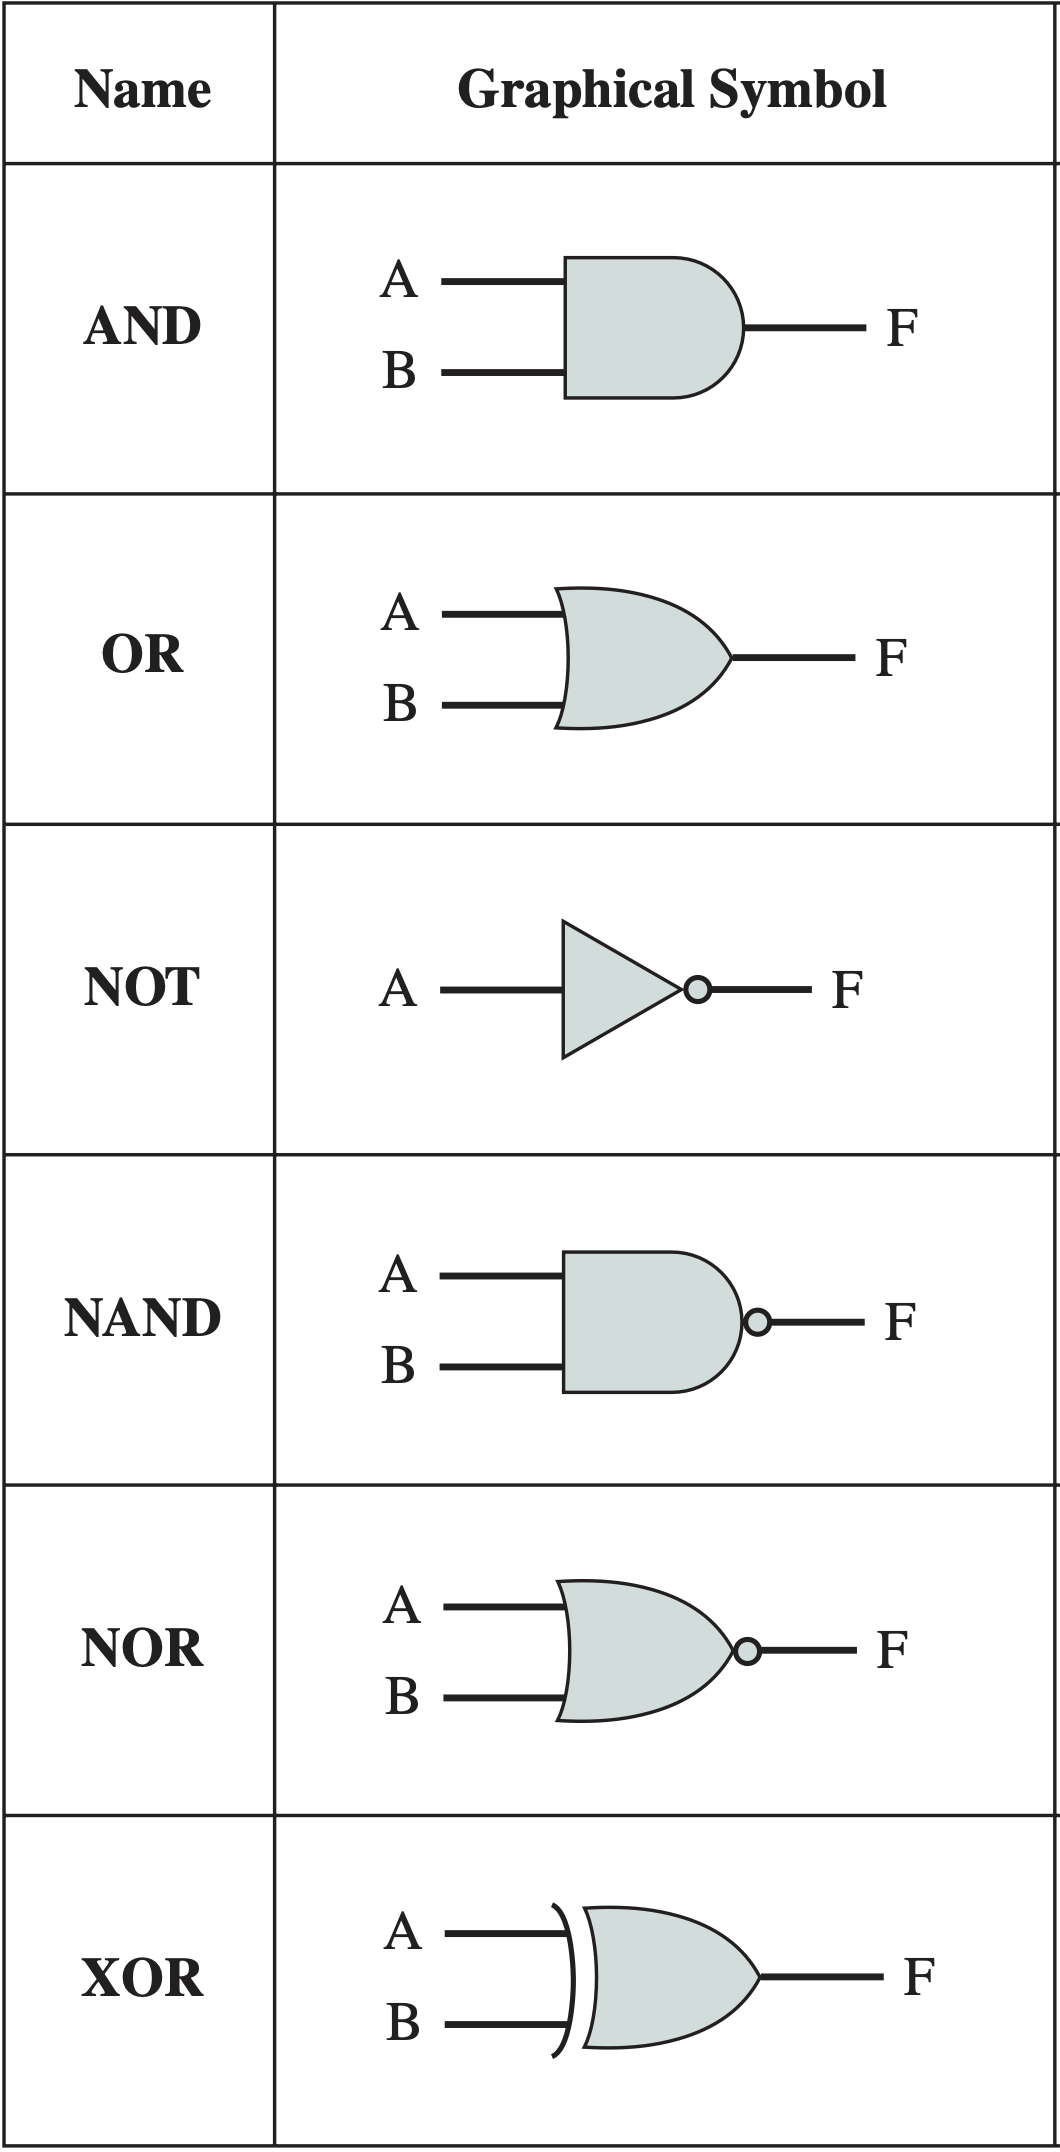
\includegraphics[scale=0.3]{chaps/digital-logic/logic-gates.png}
\end{center}

\subsection{Functional Completeness}\label{subsec:functional-completeness}
\begin{definition}[Functional Completeness]
    A set of logic gates is said to be functionally complete if any boolean function
    can be implemented using only gates from that set.
\end{definition}

\subsubsection{The \texttt{AND}, \texttt{OR}, \texttt{NOT} Set}

The set of \texttt{AND}, \texttt{OR}, and \texttt{NOT} gates is functionally complete,
i.e. they can be used to create any arbitrary boolean function.

\subsubsection{The \texttt{AND}, \texttt{NOT} Set}

By using De Morgan's Theorem, the OR operation can be implemented using only
AND and NOT gates. Therefore, this reduced set is itself functionally
complete. We start with the NAND expression in De Morgan's Theorem:
\begin{align*}
    \overline{A+B} &= \overline{A}\cdot\overline{B} \\
    \intertext{Then, we apply the NOT operation to both sides:}
    \overline{\overline{A+B}} &= \overline{\overline{A}\cdot\overline{B}} \\
    A + B &= \overline{\overline{A}\cdot\overline{B}}
\end{align*}
The left hand side is exactly the OR operation, implemented using only AND and NOT gates.

\subsubsection{The \texttt{OR}, \texttt{NOT} Set}

Similarly, by using De Morgan's Theorem, the AND operation can be implemented using only
OR and NOT gates. Therefore, this reduced set is itself functionally complete.

\subsubsection{The \texttt{NAND} Set}

The NAND operation alone can also be used to implement the AND, OR, and NOT operations.
By applying NAND between $A$ and $A$ itself, we have:
\begin{equation*}
    \overline{A\cdot A} = \overline{A} \text{ (NOT operation)}
\end{equation*}

Similarly, by applying NAND over the value of $\overline{A\cdot B}$, we have $A\cdot B$,
which is the AND operation.

Finally, by applying NAND between $\overline{A}$ and $\overline{B}$
(i.e. $\overline{\overline{A}\cdot\overline{B}}$), according to
De Morgan's Theorem, we have $A+B$, which is the OR operation.

Since AND, OR, and NOT operations can be implemented using only NAND gates,
and the set of AND, OR, and NOT gates is functionally complete, the NAND set is also
functionally complete.

\subsubsection{The \texttt{NOR} Set}

Similar to the NAND set, the NOR set is also functionally complete.

\subsection{Implementation of Boolean Functions}

Suppose we would like to implement a boolean function $F(A, B, C)$ with the following
truth table:

\begin{table}[h]
\centering
\begin{tabular}{|c|c|c||c|}
    \hline
    $A$ & $B$ & $C$ & $F(A, B, C)$ \\
    \hline
    0 & 0 & 0 & 0 \\
    0 & 0 & 1 & 0 \\
    0 & 1 & 0 & 1 \\
    0 & 1 & 1 & 1 \\
    1 & 0 & 0 & 0 \\
    1 & 0 & 1 & 0 \\
    1 & 1 & 0 & 1 \\
    1 & 1 & 1 & 0 \\
    \hline
\end{tabular}
\end{table}
The technique is to use either the Sum-of-Products (SOP) or the Product-of-Sums (POS) method.

\subsubsection{Sum-of-Products (SOP)}

SOP usually has the form of $F = XYZ + XYZ + \dots$, every term should be the product
of all the variables, appearing exactly once. Such terms are named ``minterms''.
To implement the function $F$, first identify the rows in the truth table where $F=1$,
then for each row, construct the minterm by taking the product of all the variables,
such that the sum of the minterms will give 1.

\begin{example}
    From the truth table, we observe that $F=1$ on the 3rd, 4th, and 7th rows.
    
    For the 3rd row, the product $\overline{A}B\overline{C}$ equals 1.

    For the 4th row, the product $\overline{A}BC$ equals 1.

    For the 7th row, the product $AB\overline{C}$ equals 1.

    Therefore, the function $F$ can be implemented as:
    \begin{equation*}
        F = \overline{A}B\overline{C} + \overline{A}BC + AB\overline{C}
    \end{equation*}
\end{example}

This method works because:
\begin{itemize}
    \item any other input combinations will make all the minterms 0, and the sum of 0's is 0;
    \item when one of the minterms is 1, the sum will be 1.
\end{itemize}

\subsubsection{Product-of-Sums (POS)}

Contrast to SOP, POS usually has the form of $F = (X+Y+Z)(X+Y+Z)\dots$.
The approach is to identify the rows in the truth table where $F=0$,
then for each row, construct a \textbf{product} (NOT sum) of all the variables,
such that the term give 1, then apply a NOT operation on the product. Connect all the terms
together with AND operators, and simplify using De Morgan's Theorem.

\begin{example}
    From the truth table, we observe that $F=0$ on rows other than the 3rd, 4th, and 7th.

    For the 1st row, we construct the product
    $\overline{\overline{A}\cdot\overline{B}\cdot\overline{C}}$, which equals 0.

    For the 2nd row, we construct the product
    $\overline{\overline{A}\cdot\overline{B}\cdot C}$, which equals 0.

    $\dots$

    For the 8th row, we construct the product
    $\overline{A\cdot B\cdot C}$, which equals 0.

    Then, connect the terms together with AND operations, we have:
    \begin{equation*}
        F = \left(\overline{\overline{A}\,\overline{B}\,\overline C }\right) \cdot 
            \left(\overline{\overline{A}\,\overline{B}\,          C }\right) \cdot 
            \left(\overline{          A \,\overline{B}\,\overline{C}}\right) \cdot 
            \left(\overline{          A \,\overline{B}\,          C }\right) \cdot
            \left(\overline{          A \,          B \,          C }\right)
    \end{equation*}

    For each product, apply De Morgan's Theorem
    $\overline{ABC} = \overline{A} + \overline{B} + \overline{C}$ to simplify, we have:
    \begin{equation*}
        F = (A+B+C)\cdot
            (A+B+\overline{C})\cdot
            (\overline{A}+B+C)\cdot
            (\overline{A}+B+\overline{C})\cdot
            (\overline{A}+\overline{B}+\overline{C})
    \end{equation*}
\end{example}

\begin{remark}
    Whether to use SOP or POS depends on the truth table. Generally, when there are
    less 1's in the truth table, it is easier to use SOP. When there are less 0's,
    it is easier to use POS.
\end{remark}

\subsubsection{Simplification by Boolean Algebra}

After constructing the SOP or POS expression, it is possible to simplify the expression
using the laws of boolean algebra.

\begin{example}
    The $F$ we have implemented using SOP can be simplified as follows:
\begin{align*}
    F &= \overline{A}B\overline{C} + \overline{A}BC + AB\overline{C} \\
      &= \overline{A}B\overline{C} + \overline{A}BC + \overline{A}B\overline{C} + AB\overline{C} \\
      &= \overline{A}B \left(\overline{C} + C\right) + \left(\overline{A} + A\right) B\overline{C} \\
      &= \overline{A}B + B\overline{C}
\end{align*}
\end{example}

\subsubsection{Simplification by Karnaugh Maps}

For boolean expressions with two to four variables, construct Karnaugh maps to simplify
the expression. Rule for rows and columns: adjacent rows/columns must differ by only one variable.
Rules for grouping 1's: each group-
\begin{itemize}
    \item should be as large as possible;
    \item must be rectangular in shape;
    \item must contain number of 1's that is a power of 2 (1, 2, 4, 8, etc.);
    \item can overlap or wrap around the edges;
    \item should contain at least one 1 that is not in any other groups.
\end{itemize}

\begin{example}
    To simplify $F = \overline{A}B\overline{C} + \overline{A}BC + AB\overline{C}$,
    construct the map:

    
    \begin{center}
    \begin{tabular}{rrcccc}
                                            &                                   & \multicolumn{4}{c}{\textbf{BC}}                                                                                       \\
                                            &                                   & \textbf{00}                       & \textbf{01}               & \textbf{11}               & \textbf{10}               \\ \cline{3-6} 
        \multirow{2}{*}{\textbf{A}}         & \multicolumn{1}{r|}{\textbf{0}}   & \multicolumn{1}{c|}{}             & \multicolumn{1}{c|}{}     & \multicolumn{1}{c|}{\color[HTML]{FF0000}1}    & \multicolumn{1}{c|}{\color[HTML]{6200c9}1}    \\ \cline{3-6} 
                                            & \multicolumn{1}{r|}{\textbf{1}}   & \multicolumn{1}{c|}{}             & \multicolumn{1}{c|}{}     & \multicolumn{1}{c|}{}     & \multicolumn{1}{c|}{\color[HTML]{0000FF}1}    \\ \cline{3-6} 
    \end{tabular}
    \end{center}
    
    They can be separated into two groups - one {\color[HTML]{FF0000}horizontal} and one {\color[HTML]{0000FF}vertical}.
    For the horizontal group, observe that regardless of the value of $C$, the value of $F$
    is always one, implying an expression of $\overline{A}B$. For the vertical group,
    the value of $F$ is always one regardless of the value of $A$, implying an expression of
    $B\overline{C}$. Therefore, the simplified expression is $\overline{A}B + B\overline{C}$.
\end{example}

\subsubsection{Application: Multiplexer}

\begin{example}
    Suppose we have a 2-to-1 multiplexer $s$ defined as:
    \begin{equation*}
        s = \begin{cases}
            a & \text{if } t=0 \\
            b & \text{if } t=1
        \end{cases}
    \end{equation*}
    The logical expression of the multiplexer is in fact $s = f(a, b, t)$.
    To solve for the expression, write down the truth table, and apply either SOP or POS
    to simplify the expression.
\end{example}

\subsection{Adders}

Adders can be created using logic gates. When they are chained together, they can be used
to perform addition of binary numbers. There are two types of adders:
\begin{itemize}
    \item \textbf{Half Adder}: adds two bits together, produce a sum and a carry (2-in-2-out);
    \item \textbf{Full Adder}: adds two bits and a carry produced from the previous addition,
                                produce a sum and a carry (3-in-2-out).
\end{itemize}

\subsubsection{Half Adder}

Consider the truth table of adding two digits $A$ and $B$:
\begin{table}[h]
\centering
\begin{tabular}{|c|c||c|c|}
    \hline
    $A$ & $B$ & Sum ($S$) & Carry ($C$) \\
    \hline
    0 & 0 & 0 & 0 \\
    0 & 1 & 1 & 0 \\
    1 & 0 & 1 & 0 \\
    1 & 1 & 0 & 1 \\
    \hline
\end{tabular}
\end{table}

We can observe that $S=A\oplus B$ and $C=A\cdot B$. However, the half adder cannot be used
to add numbers with more than one digit, because it does not take into account the carry
from the previous addition.

\subsubsection{Full Adder}

Now take into account the carry from the previous addition ($C'$), we have the following truth table:
\begin{table}[h]
\centering
\begin{tabular}{|c|c|c||c|c|}
    \hline
    $A$ & $B$ & $C'$ & Sum ($S$) & Carry ($C$) \\
    \hline
    0 & 0 & 0 & 0 & 0 \\
    0 & 0 & 1 & 1 & 0 \\
    0 & 1 & 0 & 1 & 0 \\
    1 & 0 & 0 & 1 & 0 \\
    1 & 1 & 0 & 0 & 1 \\
    0 & 1 & 1 & 0 & 1 \\
    1 & 0 & 1 & 0 & 1 \\
    1 & 1 & 1 & 1 & 1 \\
    \hline
\end{tabular}
\end{table}

Apply SOP, we have:
\begin{align*}
    S &= \overline{A}\overline{B}C' + \overline{A}B\overline{C'} + A\overline{B}\overline{C'} + ABC' \\
      &= C'(\overline{A}\overline{B} + AB) + \overline{C'}(\overline{A}B + A\overline{B}) \\
      &= C'(\overline{A\oplus B}) + \overline{C'}(A\oplus B) \\
      &= C'\oplus(A\oplus B)
\end{align*}
and
\begin{align*}
    C &= AB\overline{C'} + \overline{A}BC' + A\overline{B}C' + ABC' \\
      &= AB(\overline{C'} + C') + C' (\overline{A}B + A\overline{B}) \\
      &= AB + C'(A\oplus B)
\end{align*}

\section{Number Representation}

\begin{itemize}
    \item Numbers are represented in binary form in computers.
    \item Mathematical laws do not necessarily hold in computer arithmetic.
          (e.g. $3.14 + 1e20 - 1e20 \neq 3.14 + (1e20 - 1e20)$ due to precision and rounding errors)
    \item Numbers in computers are Finite Precision Numbers.
\end{itemize}

\begin{definition}[Finite Precision Numbers]\label{def:finite-precision-numbers}
    Finite Precision Numbers have the following characteristics:
    \begin{itemize}
        \item Limited number of bits to represent a number. (e.g. 32-bit integers)
        \item Limited range of numbers that can be represented. (e.g. $2^{32}$ for \texttt{unsigned int})
        \item Overflow and underflow occur when the number is too large or too small to be represented.
    \end{itemize}
\end{definition}

\subsection{Positional Number System and Radix}

\begin{definition}[Positional Number System]\label{def:positional-number-system}
    A positional number system is a system in which the position of a digit in a number determines
    its value. Numbers are represented in a string of digits in the form of:
    \begin{equation*}
        (a_na_{n-1}\ldots a_2a_1a_0.a_{-1}a_{-2}\ldots)_r
    \end{equation*}
    where:
    \begin{itemize}
        \item $n\in\mathbb{Z}$,
        \item $r\in[2, +\infty)\cap\mathbb{Z}$ is the radix (base) of the number system,
              which determines the value of each digit at position $i$ as $r^i$,
        \item $a_i\in[0, r)\cap\mathbb{Z}$.
    \end{itemize}

    The value of the number being represented is given by:
    \begin{equation}\label{eq:positional-number-system-value-direct}
        \sum_{i} (a_i r^i) \quad\text{\bfseries (The Direct Approach)}
    \end{equation}
\end{definition}

Generally, the radix value is one of 2 (binary), 8 (octal), 10 (decimal), or 16 (hexadecimal).

\begin{example}
    The number 1A6.BE$_{16}$ is a fractional number in hexadecimal system. Its value in decimal system is:
    \begin{align*}
        \text{1A6.BE}_{16} &=
            1\times 16^2 + 10\times 16^1 + 6\times 16^0 + 11\times 16^{-1} + 14\times 16^{-2} \\
            &= 422.7421875_{10}
    \end{align*}
\end{example}

\begin{theorem}[Iterative Approach of Evaluating the Value of a Positional Number]
    The value of a number in a positional number system can be evaluated alternatively by:
    \begin{equation}\label{eq:positional-number-system-value-iterative}
        r\left(r\left(r\left(r\cdot a_n + a_{n-1}\right)+ a_{n-2}\right)+ a_{n-3} \dots\right) + a_0
        \quad \text{\bfseries (The Iterative Approach)}
    \end{equation}
    which is more efficient than the direct approach.
\end{theorem}

\begin{proof}
    Consider only the integer case.
    For the direct approach, for each digit $a_i$, its value is calculated by \[
        a_i \underbrace{\times r \times r \times \dots \times r}_{i\text{ times}}
    \] Therefore, for $i=n$, the number of multiplications performed is $n$ times.
    The total number of multiplications performed to convert a number of $n$ digits is \[
        1+2+3+\dots+n = \frac{n(n+1)}{2} = O(n^2)
    \]

    For the iterative approach, the left most digit ($a_n$) is first multiplied by $r$ and added to
    the next digit ($a_{n-1}$). This sum is then multiplied by $r$ and added to the next digit
    ($a_{n-2}$), and so on. The total number of multiplications performed is $n$ times. Therefore,
    the iterative approach has a linear complexity $O(n)$.

    Hence, the iterative approach is more efficient than the direct approach.
\end{proof}

\subsection{Integer Representation}

\subsubsection{Unsigned Integer Representation}

\begin{definition}
    For a sequence of $n$ bits ($a_{n-1}a_{n-2}\ldots a_1a_0$), it represents a nonnegative integer
    of value A, where
    \begin{equation*}
        A = \sum_{i=0}^{n-1} 2^i a_i
    \end{equation*}
\end{definition}

\subsubsection{Sign-and-Magnitude Representation}

\begin{definition}
    For a sequence of $n$ bits, the MSB\footnotemark is used
    to represent the sign of the number. The rest $n-1$ bits represent the magnitude of the number.
    The value of the number is given by:
    \begin{equation*}
        A = (-1)^{a_{n-1}} \sum_{i=0}^{n-2} 2^i a_i
    \end{equation*}

    \begin{example}
    For 4-bit integers, we have:
    \begin{align*}
        \boldsymbol{0}0110101_2 &= \boldsymbol{+}53_{10} \\
        \boldsymbol{1}0110101_2 &= \boldsymbol{-}53_{10}
    \end{align*}
    \end{example}

\end{definition}

\footnotetext{Most Significant Bit (the leftmost bit)}

This representation has two pitfalls:
\begin{enumerate*}
    \item It has two representations for zero ($0000_2$) and ($1000_2$).
    \item It is inconvenient for arithmetic operations.
\end{enumerate*}
Therefore, this representation is rarely used to represent integers.

\subsubsection{One's and Two's Complement Representation}

\begin{definition}[One's Complement]
    For each positive integer, its one's complement representation is unchanged. For each negative
    number, its one's complement representation is obtained by flipping all the bits of its
    corresponding positive number.

    \begin{example}
        For 8-bit representation of $+8$, its one's complement is $0000\,1000_2$.
        For $-8$, its one's complement is obtained by flipping every bit of +8, which is $1111\,0111_2$.
    \end{example}
\end{definition}

One's Complement representation still has two representations for zero ($0000_2$) and ($1111_2$).
Therefore, Two's Complement representation is more commonly used.

\begin{definition}[Two's Complement]
    For each positive integer, its two's complement representation is unchanged. For each negative
    number, its two's complement representation is obtained by adding 1 to its one's complement.

    \begin{example}
        For 8-bit representation of $+13$, its two's complement is $0000\,1101_2$. For $-13$, its
        two's complement is obtained by adding 1 to its one's complement, which is
        $1111\,0010_2 + 0000\,0001_2 = 1111\,0011_2$.
    \end{example}

    \begin{equation*}
        A = -2^{n-1}a_{n-1} + \sum_{i=0}^{n-2} 2^i a_i
    \end{equation*}
\end{definition}

For the ``negative zero'', by the definition of two's complement, its 8-bit representation will be
$-0_{10} = 1111\,1111_2 + 0000\,0001_2 = 1\,0000\,0000_2$. However, since the result is 9 bits, the
carry bit is discarded, and the result is $0000\,0000_2$, which is the same as the representation of
the ``positive zero''. The two's complement has only one representation for zero.

For arithmetic operations, simply add the two numbers together, and discard any carry from the MSB,
the result will be the correct answer.

\begin{remark}
    Like the Sign-and-Magnitude representation, the One's and Two's Complement representations use
    the MSB as the sign bit.
\end{remark}

\begin{theorem}[Overflow Rule for Two's Complement]\label{thm:overflow-rule-twos-complement}
    When two numbers of the same sign are added, overflow occurs iff the result has an opposite sign.
\end{theorem}

\subsubsection{Range Extension}

It is sometimes useful to store an integer that requires $n$ bits in $m$ bits ($m>n$). Different
methods are needed for different representations.

\begin{itemize}
    \item \textbf{Unsigned Integer}: Add more bits to the left and fill them with zeros.
    \item \textbf{Sign-and-Magnitude}: Add more bits to the left. Move the sign bit to the new MSB,
            and fill the rest with zeros.
    \item \textbf{Two's Complement}: Add more bits to the left. Fill the new bits with the sign bit.
            (\textbf{Sign Extension})
\end{itemize}

\subsection{Integer Arithmetic Operations}

\subsubsection{Negation of Two's Complement}

\begin{definition}[Negation of Two's Complement]
To negate a number in Two's Complement representation, take the Two's Complement of the number.
\end{definition}

\subsubsection{Addition and Subtraction}

Addition of two numbers in Two's Complement is the same as if they were unsigned integers.
Refer to Theorem \ref{thm:overflow-rule-twos-complement} for overflow rule. For subtraction,
negate the second operand and perform addition.

\subsubsection{Multiplication}

To make explanations clear, we call the first operand the \textbf{multiplicand} and the second
operand the \textbf{multiplier}.

For \textbf{unsigned integers}, perform:
\begin{enumerate}
    \item For the $i$-th bit of the multiplier, if it is 1, shift the multiplicand left
        by $i$ bits and add it to the partial sum. ($a_i$ as in $a_na_{n-1}\ldots a_1a_0$)
    \item If the $i$-th bit of the multiplier is 0, do nothing.
    \item Return the partial sum as the result.
\end{enumerate}

For \textbf{two's complement integers with both operands being positive}, perform the same 
steps as for unsigned integers.
For \textbf{two $n$-bit two's complement integers with one or both operands being negative},
perform:
\begin{enumerate}
    \item For the $i$-th bit of the multiplier, where $i\in[0, n-1]$, if it is 1, shift the
        multiplicand left by $i$ bits, then sign-extend it to $2n$ bits, and add it to the 
        partial sum.
    \item For the MSB of the multiplier,
        \begin{itemize}
            \item If it is 1, take the two's complement of the multiplicand, sign-extend it
                to $2n$ bits, and add it to the partial sum.
            \item If it is 0, do nothing.
        \end{itemize}
    \item Sum the partial sums, ignore the carry bit, and return the result.
\end{enumerate}

\begin{example} [Multiplication of $-11$ and $-13$ in 8-bit two's complement]
    \begin{equation*}\begin{aligned}[t]\begin{arithmetic}[t]
                1111\,0011 &    (multiplicand $-13$) \\
        \times  1111\,0101 &    (multiplier $-11$)   \\
    1111\,1111\,1111\,0011 &    (left shift by 0, sign-extend) \\
    1111\,1111\,1100\,11~~ &    (left shift by 2, sign-extend) \\ 
    1111\,1111\,0011\,~~~~ &    $\cdots$ \\
    1111\,1110\,011~\,~~~~ \\
    1111\,1100\,11~~\,~~~~ \\
  + 0000\,0110\,1~~~\,~~~~ &    (two's complement of multiplicand, sign-extend) \\
    \cancel{101}\,0000\,0000\,1000\,1111 & (product $+143$)\\
    \end{arithmetic}\end{aligned}\end{equation*}
\end{example}

\begin{theorem}
    Multiplying an $n$-bit integer by an $m$-bit integer
    produces a product of at most $(n+m)$ bits.
\end{theorem}

\subsubsection{Division}

\textit{Not covered in this course.}

\subsection{Floating-Point Representation}

\subsubsection{Excess-$K$ (Bias) Representation}

\begin{definition}[Excess-$K$ Representation]
    In an $n$-bit Excess-$K$ representation, the values that are represented are in the interval of
    $[0 - K, 2^n - 1 - K]$, where the smallest value is represented by all bits being 0, and the
    greatest value is represented by all bits being 1.

    The $K$ is referred to an offset, or bias, as it is subtracted from the \textit{bit pattern value} to
    obtain the represented \textit{true value}.

    \begin{example}
        In a 3-bit Excess-5 representation, we have:

        \centering
        \begin{tabular}{|c|c|c|}
            \hline
            Bit Pattern & Bit Pattern Value & True Value \\
            \hline
            111 & 7 & 2 ($=7-5$) \\
            110 & 6 & 1 \\
            101 & 5 & 0 \\
            100 & 4 & -1 \\
            011 & 3 & -2 \\
            010 & 2 & -3 \\
            001 & 1 & -4 \\
            000 & 0 & -5 \\
            \hline
        \end{tabular}
    \end{example}

    The $K$ is typically chosen to be $2^{n-1}$ or $2^{n-1} - 1$, with the latter being more common.

    The Excess-$2^{n-1} - 1$ representation is used for representing a floating-point number
    as regulated by the IEEE\footnotemark standard.
\end{definition}

\footnotetext{Institute of Electrical and Electronics Engineers}

\subsubsection{IEEE 754-2008 Floating-Point Number Representation}

\begin{definition}[Format of a Floating-Point Number]
    A floating-point number is represented in the form of:
    \[\pm\,\text{Significand}\times 2^{\,\pm\,\text{(Biased) Exponent}}\]
\end{definition}

In a general 32-bit IEEE floating-point number, it is stored in memory by:

\begin{center}
    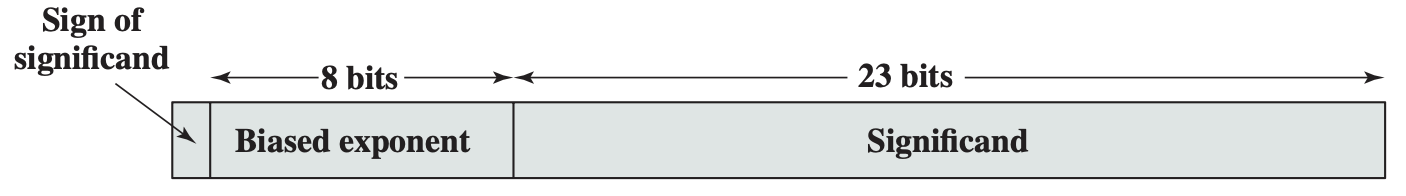
\includegraphics[scale=0.5]{chaps/number-representation/32-bit-ieee-float.png}
\end{center}

The floating-point number is always normalised before being stored. A normal number is the one
with the MSB being 1. The convention is to always make the radix point to the right of the MSB,
i.e. the MSB is always 1. Therefore, the MSB is never stored in memory. A normal nonzero number
takes the form:
\[\pm 1.\underbrace{\text{bbb}\ldots\text{b}}_{\text{23 bits}}\times 2^{\,\pm\,\text{E}}\]

The exponent is stored in Excess-$127$ ($2^{8-1} - 1$). Meaning that 127 is added to the true
exponent before being stored.

Note that since there is always a leading 1, the significand is always in the range of $[1, 2)$.
This implies that when the floating-point number is too far away from or too close to zero, it
cannot be represented accurately. The following diagram shows the range of representable values
of a 32-bit floating-point number (\textbf{not the IEEE standard}):

\begin{center}
    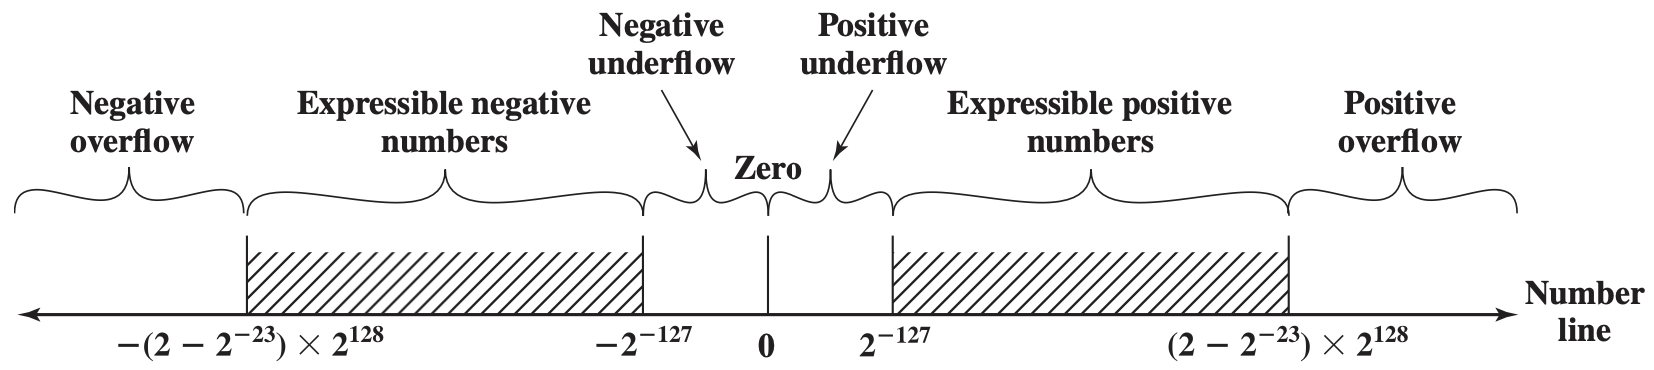
\includegraphics[scale=0.5]{chaps/number-representation/32-bit-ieee-float-range.png}
\end{center}

The diagram shows 0 is in the range of underflow, which can be inconvenient. Therefore, special
values are defined in the IEEE standard
to represent 0, $\pm\infty$, and \texttt{NaN} (Not a Number).
\begin{itemize}
    \item $\pm0$: Biased exponent and significand are all 0. The sign bit determines the sign.
    \item $\pm\infty$: Biased exponent is all 1, and significand is all 0.
    \item \texttt{NaN}: Biased exponent is all 1, and significand is not all 0.
    \item Subnormal numbers: Biased exponent is all 0, and significand is not all 0.
        ($\pm 2^{-126}(0.\text{S})$) Allows gradual underflow.
\end{itemize}

\begin{remark}
    In assignments and exams, unless specified, the above special meanings are not considered.
\end{remark}

IEEE 754-2008 defines three types of binary floating-point numbers - 
single precision (\texttt{Binary32}), double precision (\texttt{Binary64}), and
quadruple precision (\texttt{Binary128}). The following table shows the parameters of each type:

\begin{center}
    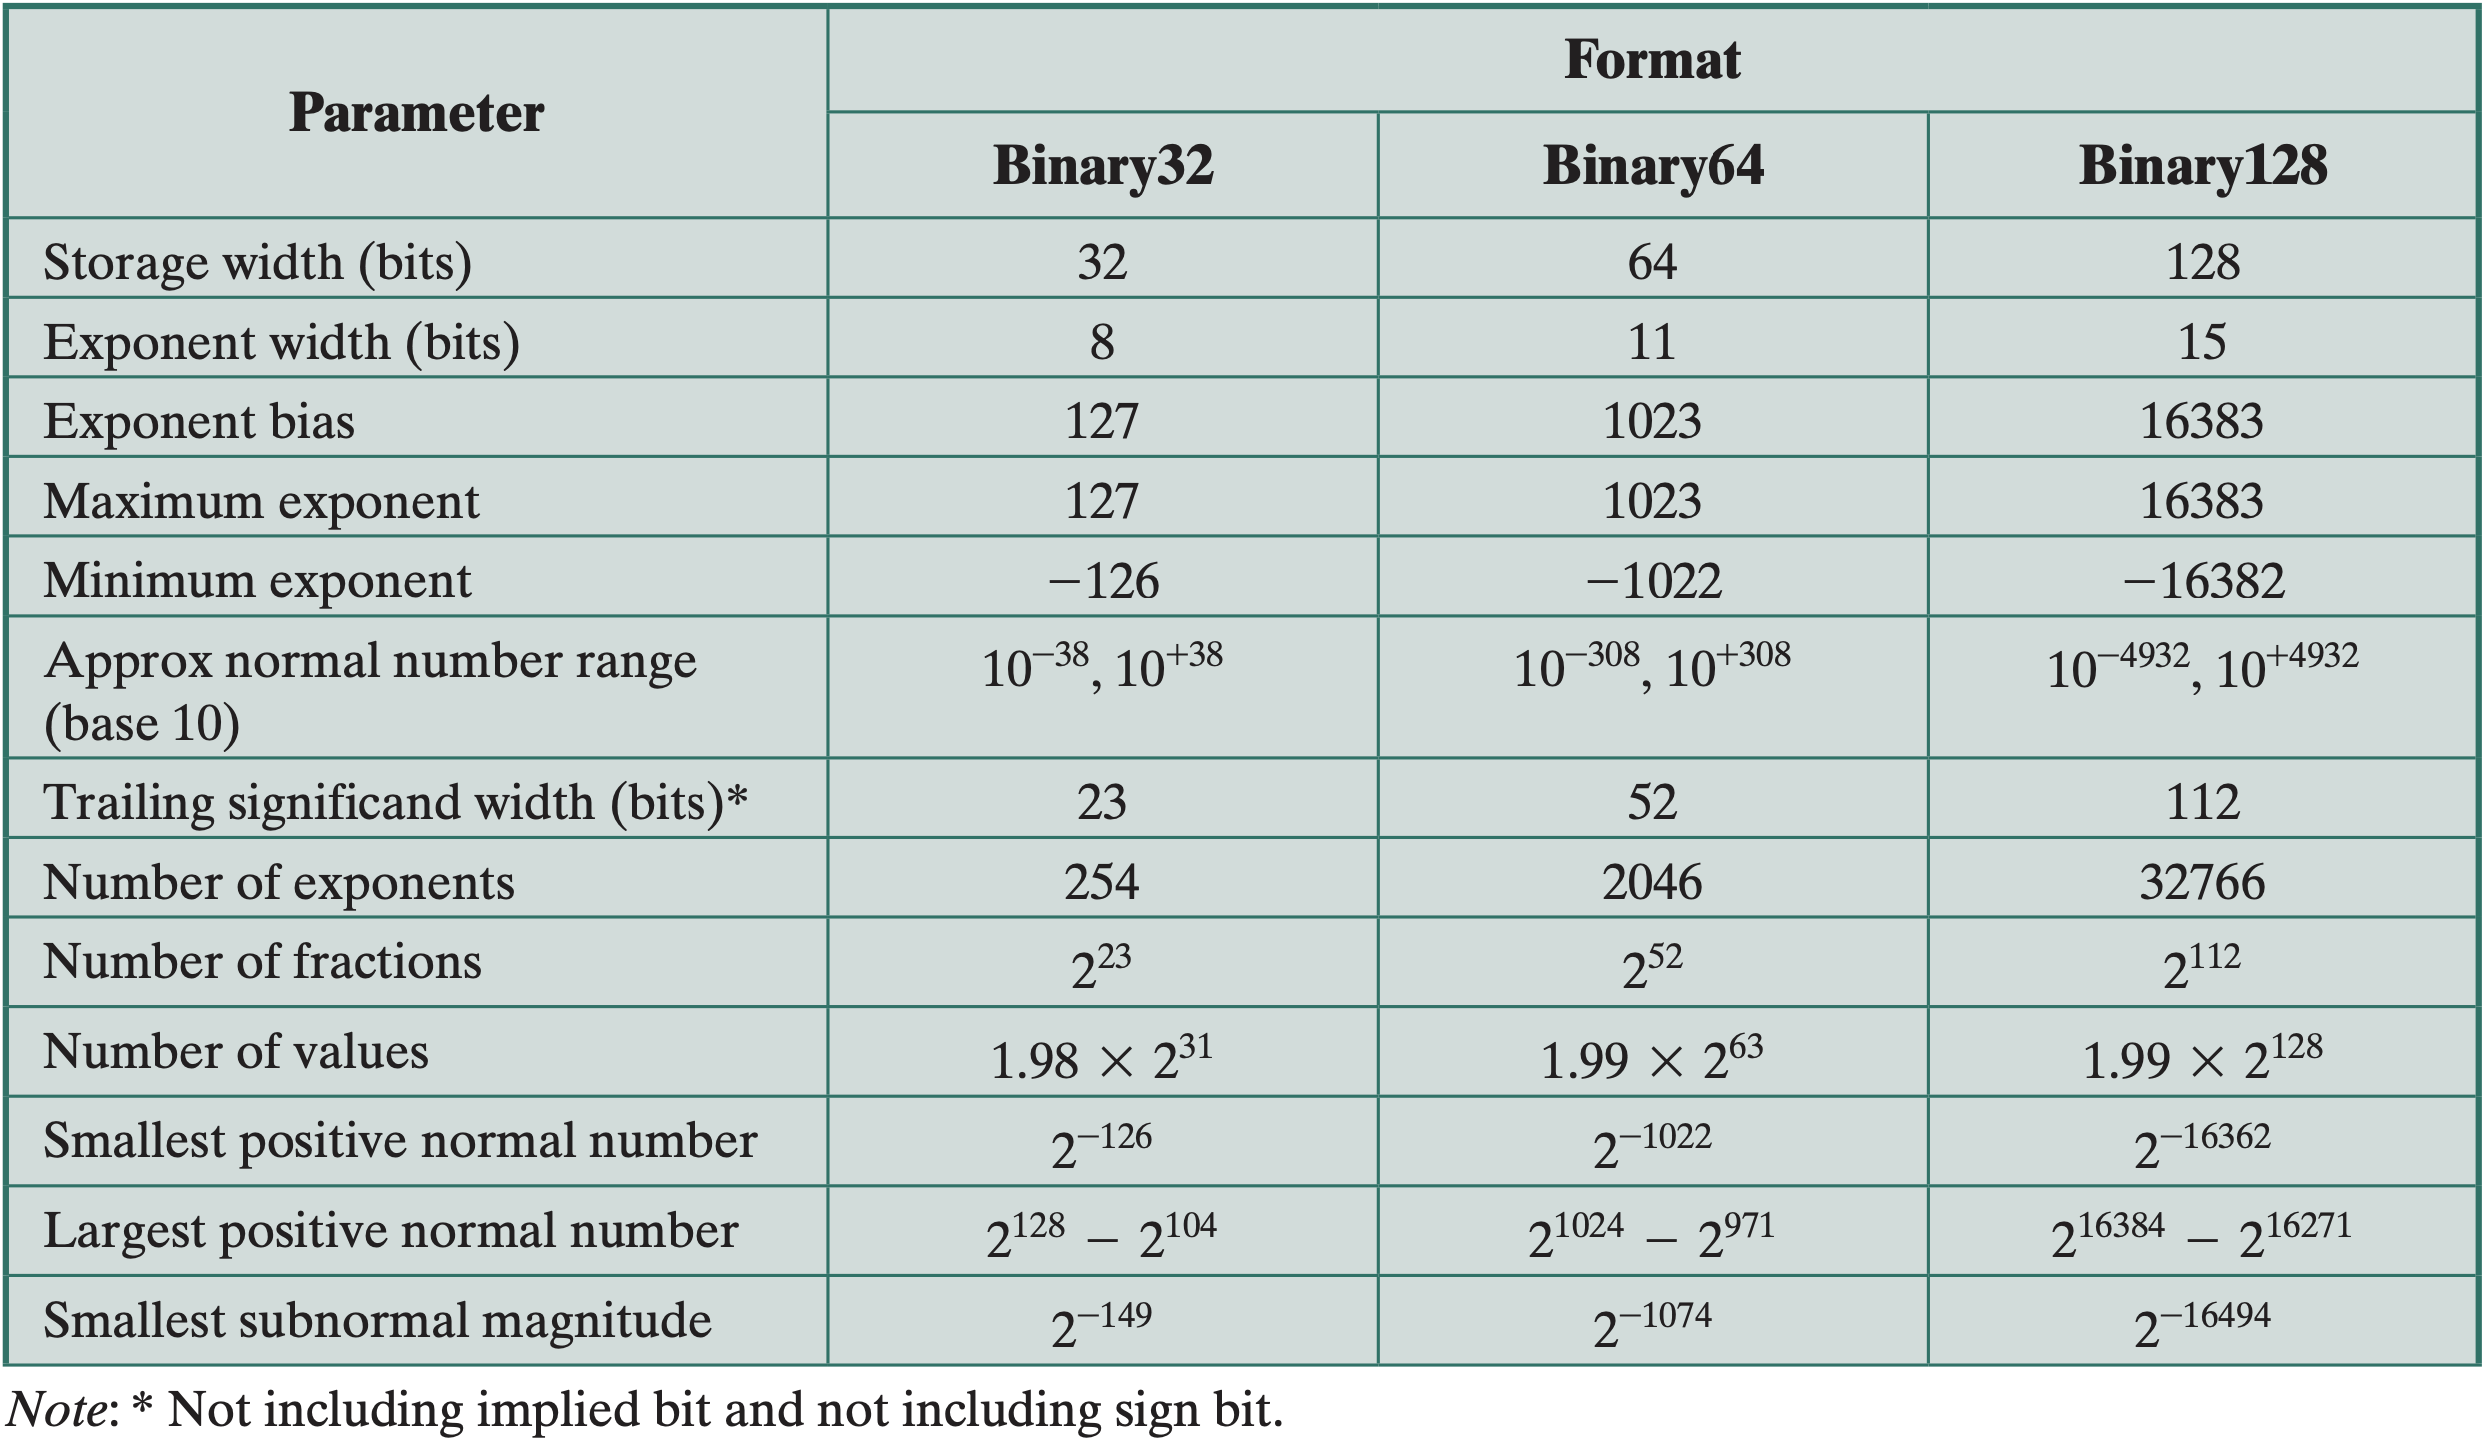
\includegraphics[scale=0.3]{chaps/number-representation/ieee-754-binary-float-parameters.png}
\end{center}

\begin{example}[Manual conversion of a decimal number to Binary32 floating-point number]
    To convert -23.875 to a 32-bit floating-point number, we have these steps:
    \begin{itemize}
        \item Convert -23.875 to binary: $-23.875_{10} = -10111.111_2$
        \item Normalise the binary number: $-10111.111_2 = -1.0111111_2\times 2^4$
        \item Convert the exponent to biased exponent: $4 + 127 = 131 = 10000011_2$
        \item Set the sign bit, biased exponent, and significand:
            $\boxed{\underbrace{1}_{\text{sign}}\,\underbrace{1000\,0011}_{\text{biased exponent}}\,
            \underbrace{0111\,1110\,0000\,0000\,0000\,000}_{\text{significand}}}$
    \end{itemize}
\end{example}

\begin{theorem}
    Some important properties of floating-point numbers:
    \begin{itemize}
        \item The number of representable values of a $n$-bit floating-point number is
            NOT greater than that of a $n$-bit integer (both being $2^n$).
        \item The representable values of a floating-point number are NOT uniformly distributed.
    \end{itemize}
\end{theorem}

\subsection{Floating-Point Arithmetic Operations}

\subsubsection{Addition and Subtraction}

Steps for floating-point number addition and subtraction:
\begin{enumerate}
    \item For the number with the smaller exponent, shift the significand right by the difference
        in the exponents to align their radix points.
    \item Add or subtract the significands, then determine the sign of the result.
    \item Normalise the result. Truncate the significand to the largest number of bits allowed.
\end{enumerate}

Generally, there are five phrases in floating-point addition and subtraction:
\begin{enumerate}
    \item \textbf{Check for zeros};
    \item \textbf{Alignment} of significands;
    \item \textbf{Addition/Subtraction} of significands;
    \item \textbf{Normalisation} of the result;
    \item \textbf{Rounding}.
\end{enumerate}

A typical floating-point addition/subtraction is illustrated in the following flowchart:

\begin{figure}[H]
    \centering
    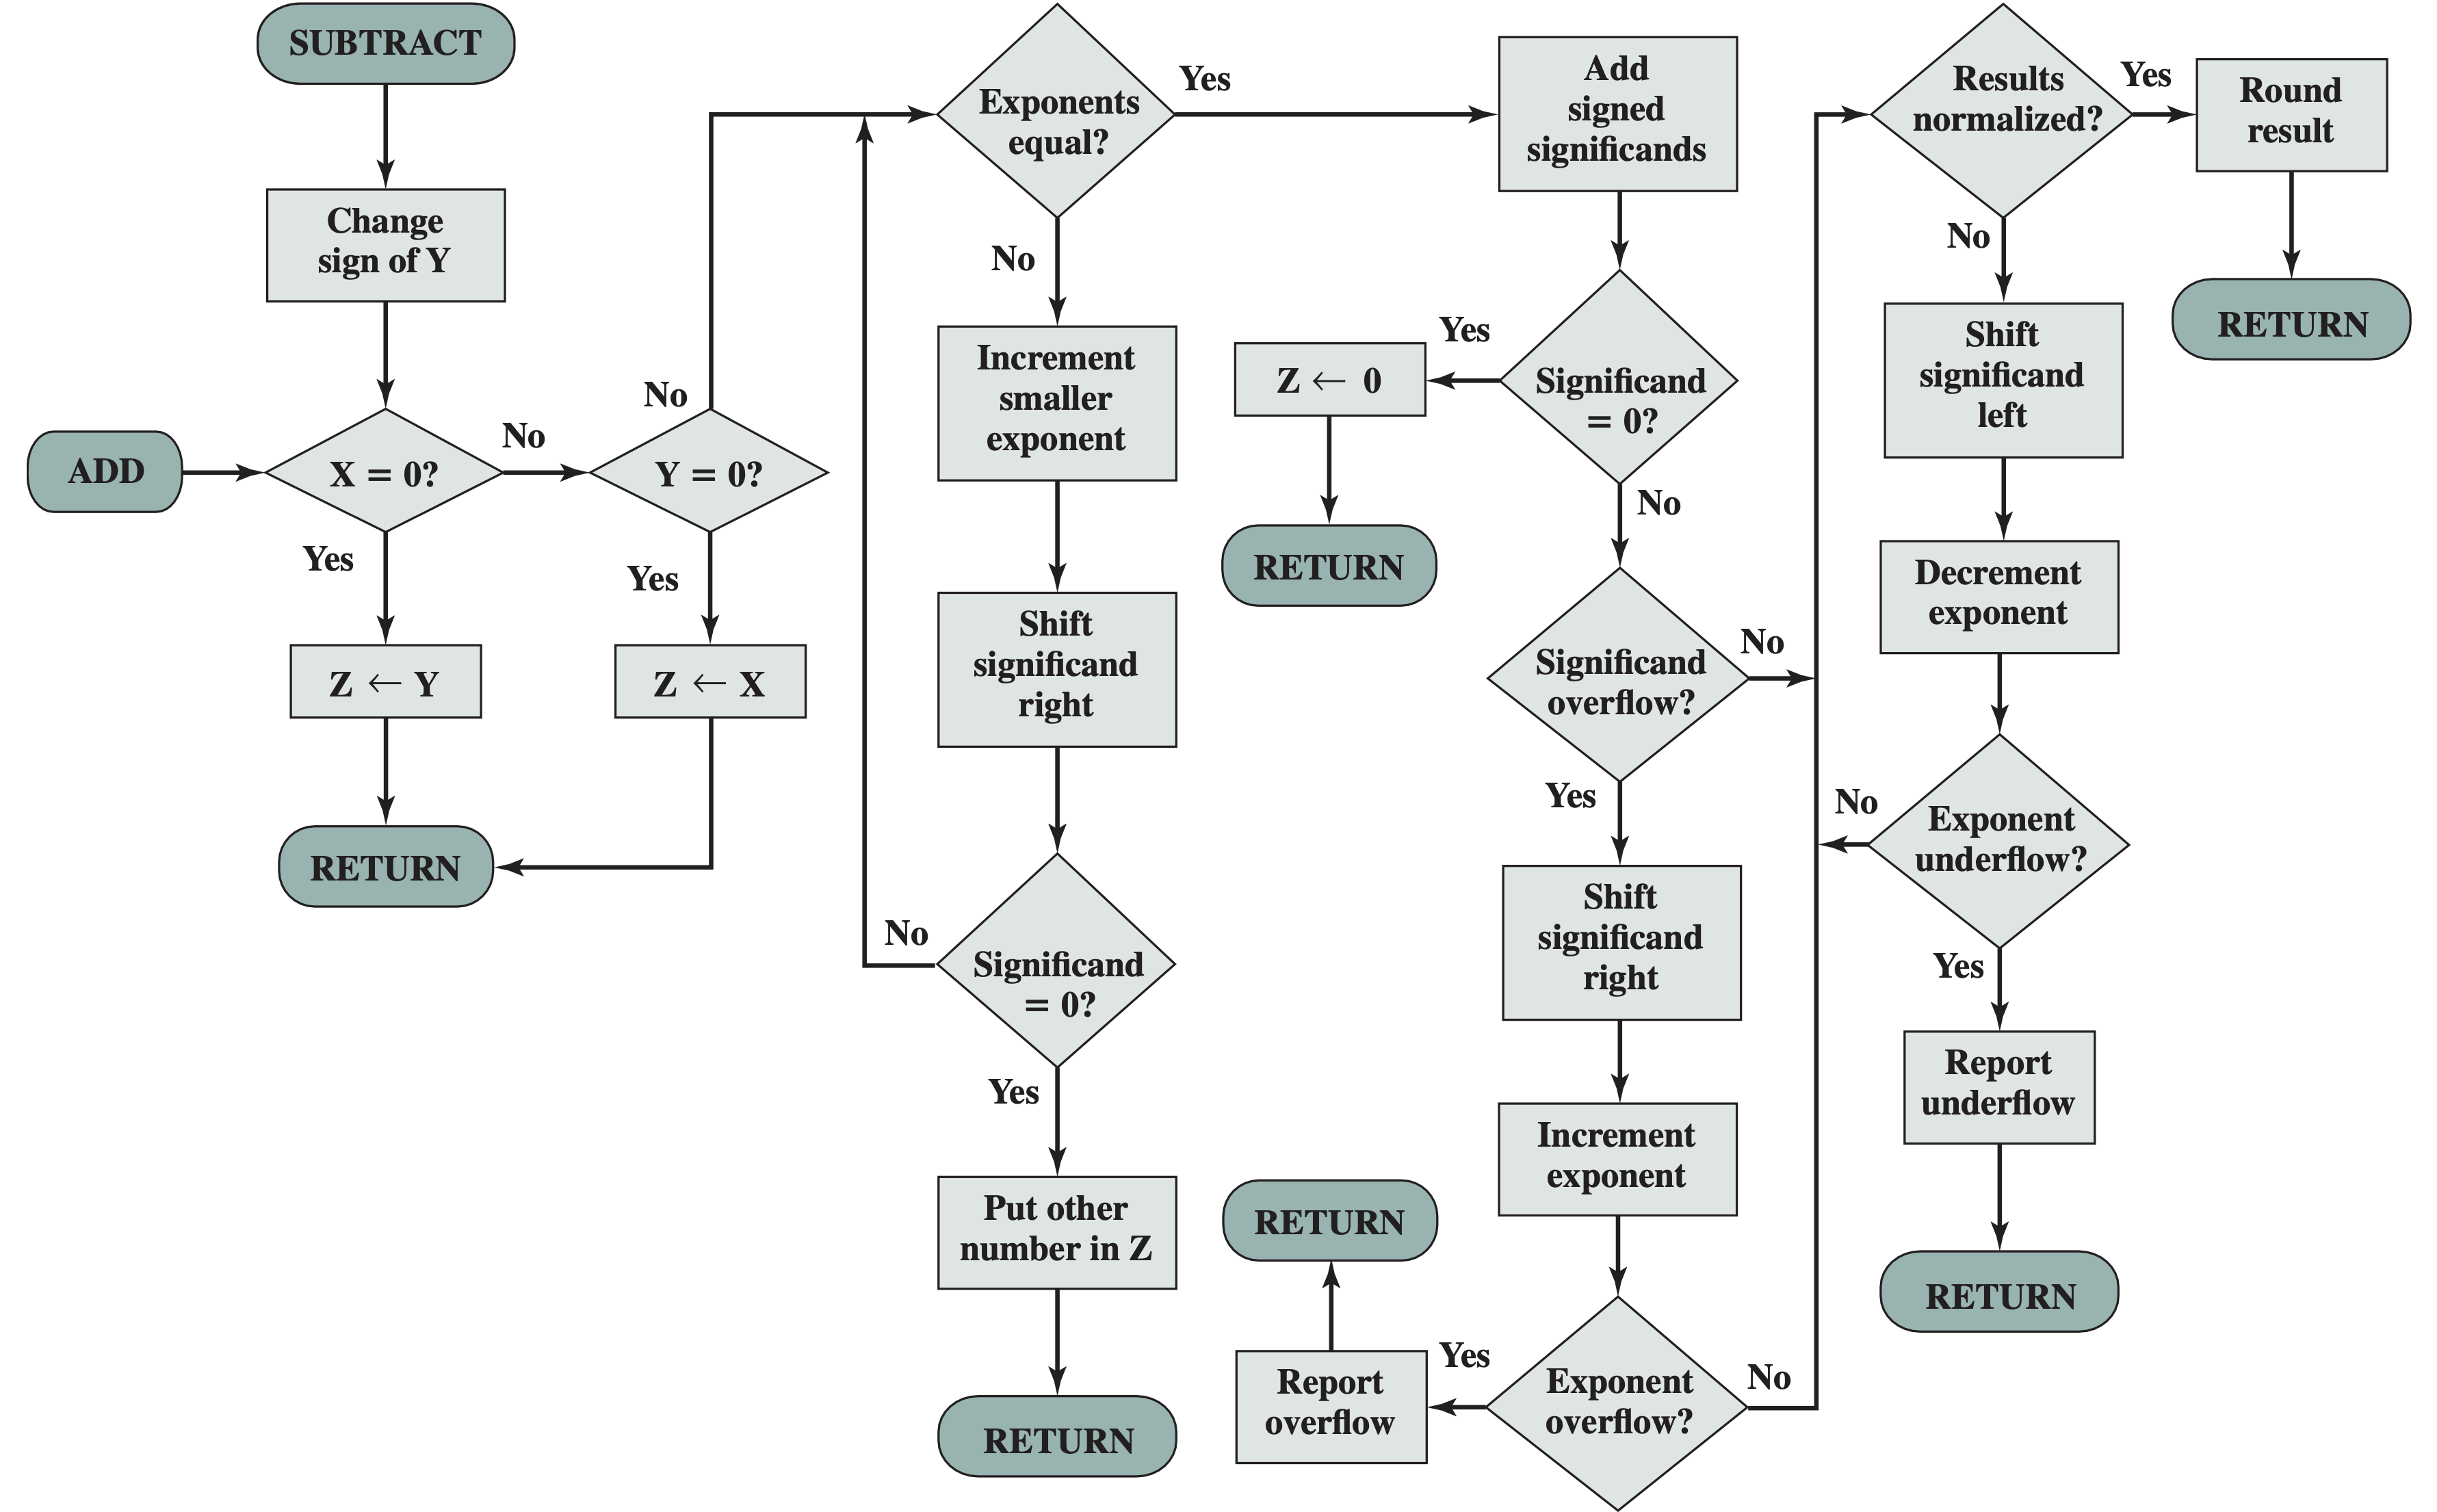
\includegraphics[scale=0.29]{chaps/number-representation/flt-add-sub-flow-chart.png}
    \caption{Floating-Point Addition and Subtraction Flowchart}
\end{figure}

\subsubsection{Multiplication}

Consider the multiplication illustrated in the equation:
\begin{equation*}
    \pm m_1\times 2^{\text{exp}_1} \times \pm m_2\times 2^{\text{exp}_2} =
    \pm m_1\times m_2\times 2^{\text{exp}_1 + \text{exp}_2}
\end{equation*}
where $\text{exp}$ is the real exponent value stored in Excess-$K$, whose bit pattern is
$\text{e} := \text{exp} + K$. To perform multiplication, the exponents are added, and the
significands are multiplied. The result is then normalised.

Consider the addition of the exponents' bit pattern, we have:
\begin{align*}
    \text{exp}_1 + \text{exp}_2 &= (\text{e}_1 - K) + (\text{e}_2 - K) \\
    \text{exp}_\text{sum} &= \text{e}_1 + \text{e}_2 - 2K \\
    \text{e}_\text{sum} - K &= \text{e}_1 + \text{e}_2 - 2K \\
    \text{e}_\text{sum} &= \text{e}_1 + \text{e}_2 - K
\end{align*}
Therefore, the bias $K$ is subtracted from the sum of the exponents' bit patterns.
Then, determine the sign of the result, and normalise and round the result.

\subsubsection{Division}

Division of floating-point numbers is similar to multiplication. It is defined by:
\begin{equation*}
    \frac{\pm m_1\times 2^{\text{exp}_1}}{\pm m_2\times 2^{\text{exp}_2}} =
    \pm \frac{m_1}{m_2}\times 2^{\text{exp}_1 - \text{exp}_2}
\end{equation*}

For the division of the exponents' bit patterns, we have:
\begin{align*}
    \text{exp}_1 - \text{exp}_2 &= (\text{e}_1 - K) - (\text{e}_2 - K) \\
    \text{exp}_\text{diff} &= \text{e}_1 - \text{e}_2 \\
    \text{e}_\text{diff} - K &= \text{e}_1 - \text{e}_2 \\
    \text{e}_\text{diff} &= \text{e}_1 - \text{e}_2 + K
\end{align*}
Therefore, the bit patterns of the exponents are subtracted, and the bias $K$ is added to the result.
Then, determine the sign of the result, and normalise and round the result.

Flowcharts showing floating-point multiplication and division are shown below.

\begin{figure}[H]
    \centering
    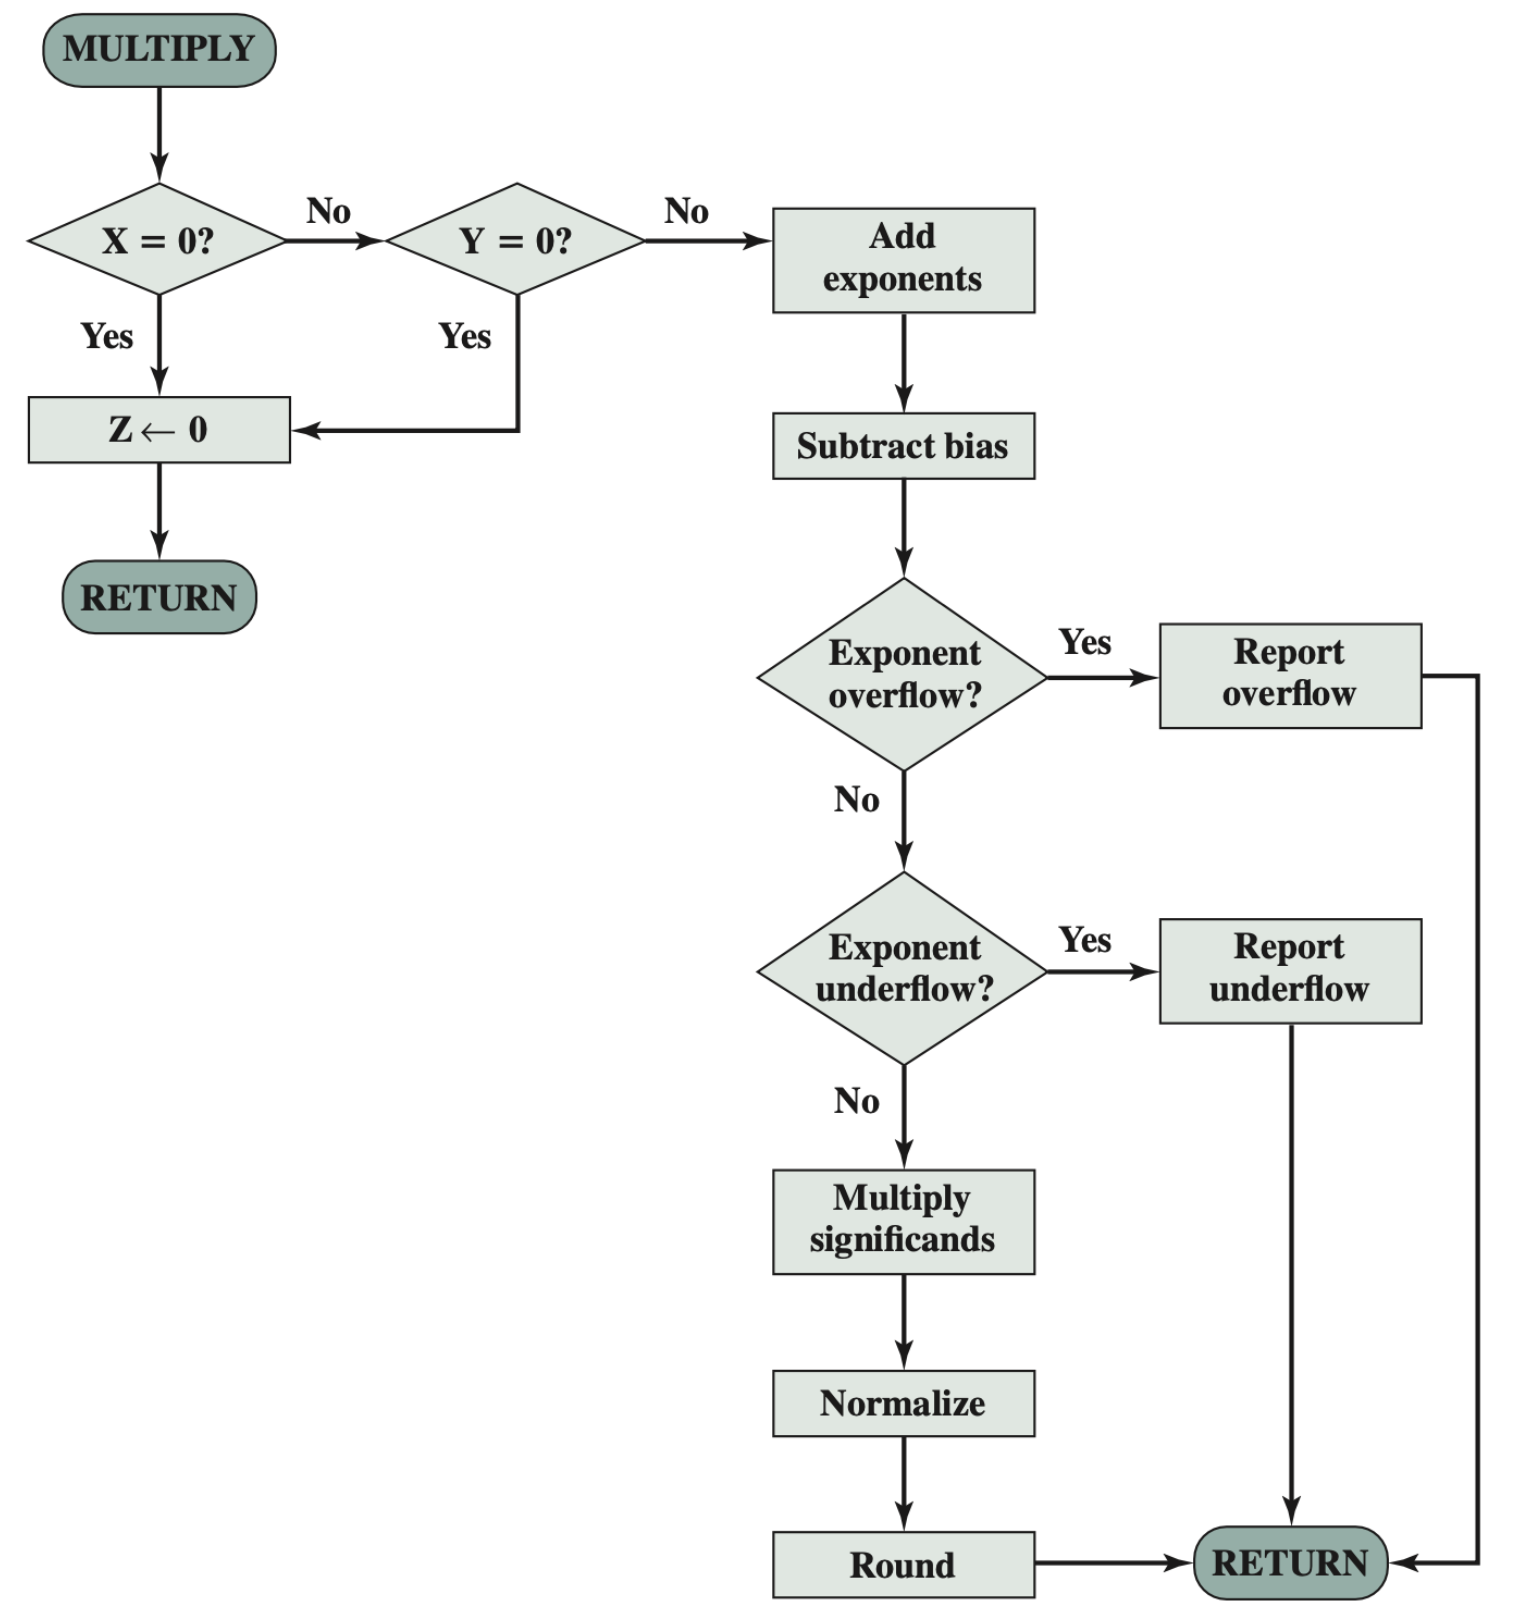
\includegraphics[width=0.45\linewidth]{chaps/number-representation/flt-multiply-flowchart.png}
    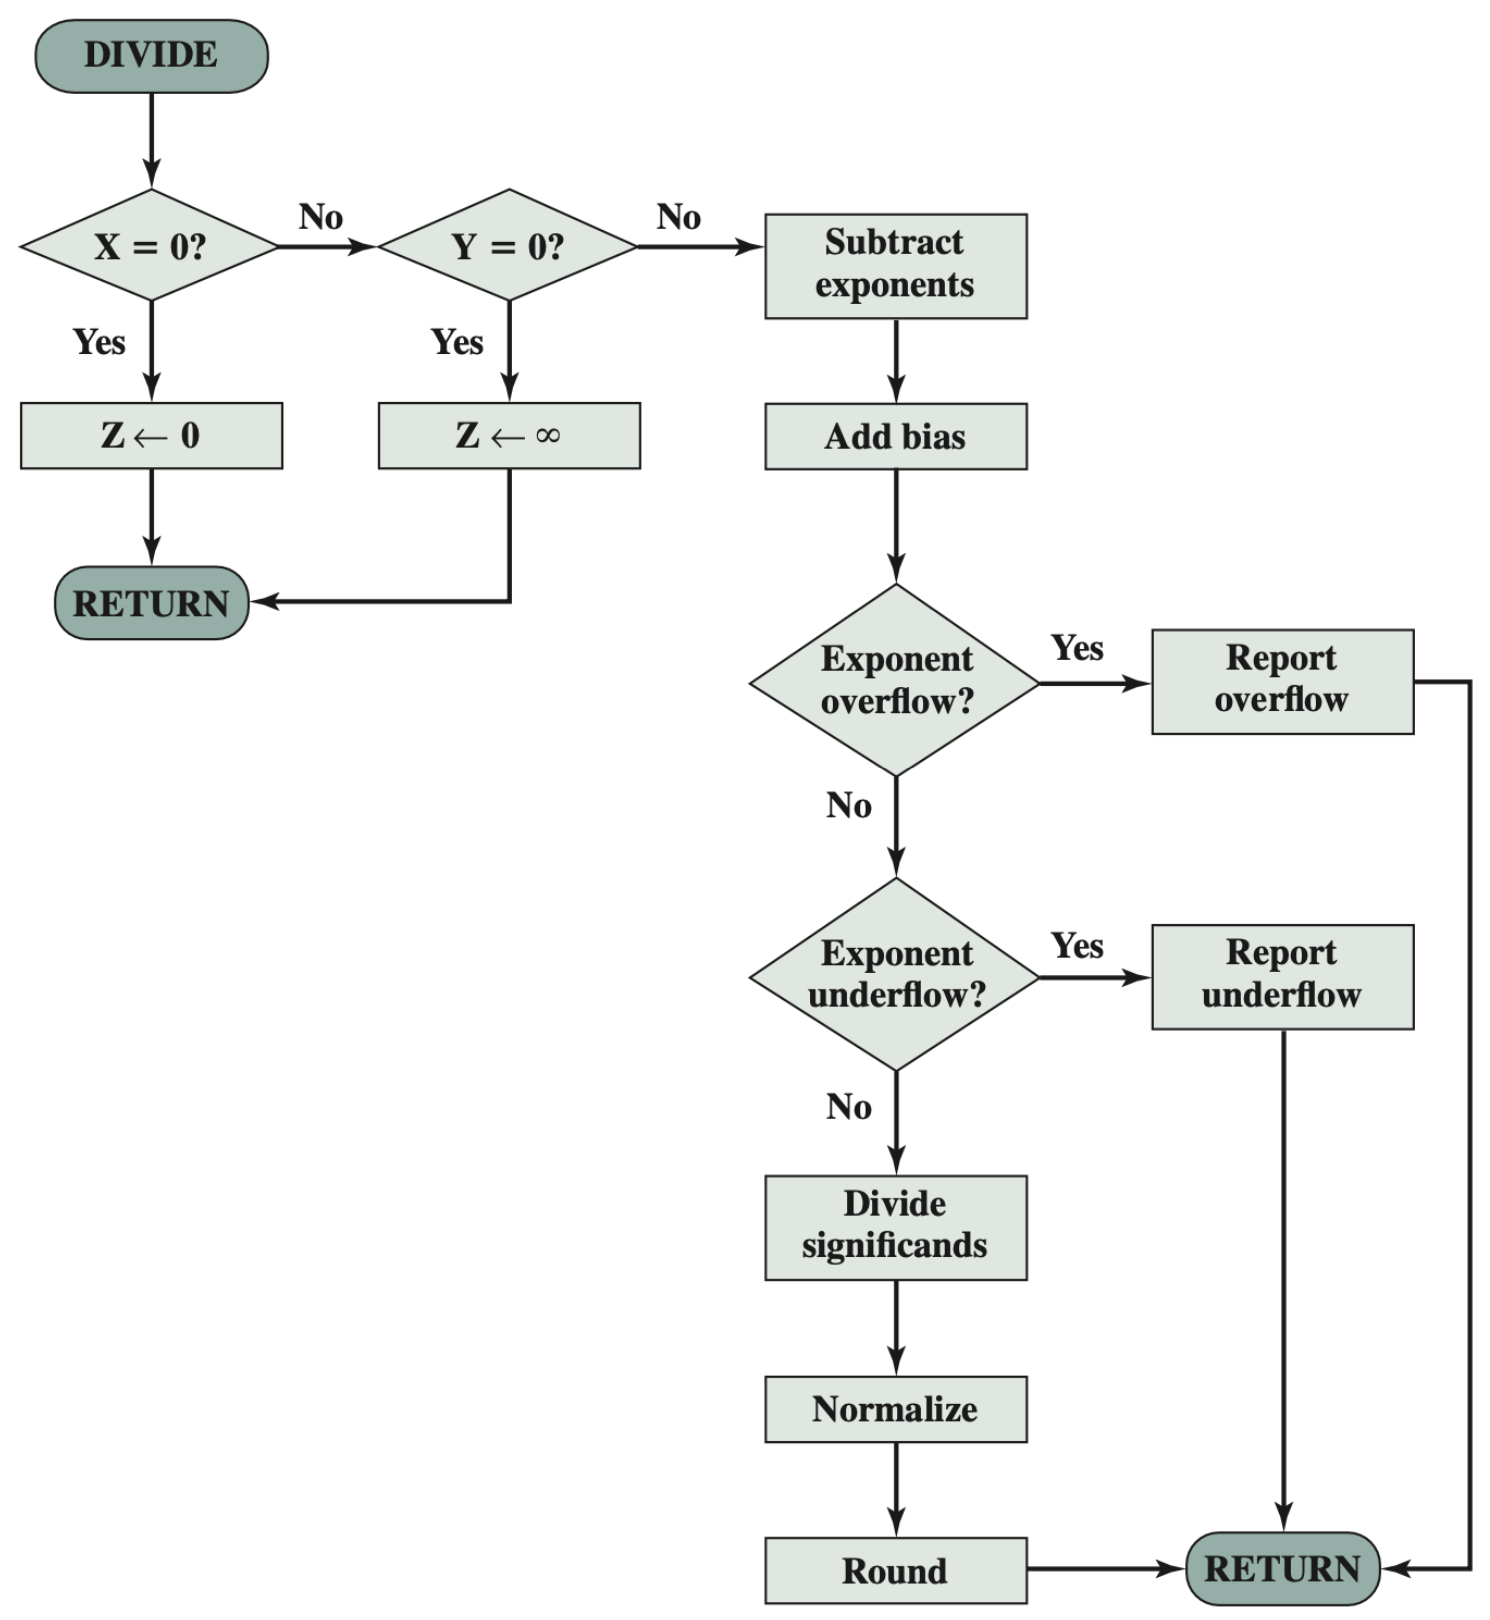
\includegraphics[width=0.45\linewidth]{chaps/number-representation/flt-divide-flowchart.png}
    \caption{Floating-Point Multiplication and Division Flowcharts}
\end{figure}

\subsubsection{Approximation of Floating-Point Arithmetic}

Floating-point numbers are prone to precision errors due to the following reasons:
\begin{itemize}
    \item Not all numbers can be represented precisely in binary,
        e.g. $0.2_{10} = $0.00110011\ldots$_2$.
    \item Round-off errors: some digits of the significand is lost to the left or right end
        of the significand when being shifted.
\end{itemize}

Due to errors, the Associative Law do not necessarily hold, especially when a very large number
is calculated with a very small number. In such cases, different orders of operations may yield
different results.

Different approaches for rounding a floating-point number include
\begin{enumerate*}
    \item round to nearest,
    \item round towards zero,
    \item round towards $\pm\infty$.
\end{enumerate*}

\section{Instruction Execution Cycle}

\subsection{Terminologies and Basic Information}

Terminologies:
\begin{itemize}
    \item \textbf{Byte}: 8 bits, smallest addressable unit of memory.
    \item \textbf{Word}: Unit of organisation of memory, varies from system to system.
        e.g. 32-bit, 64-bit, etc.
    \item \textbf{Register}: Small, fast storage location within the CPU.
    \item \textbf{Word Addressing}: Addressese of memory on a computer that uniquely
        identify a word.
    \item \textbf{Byte Addressing}: Addresses of memory on a computer that uniquely
        identify a byte.
\end{itemize}

Registers inside a CPU:
\begin{itemize}
    \item \textbf{PC (Program Counter)}: Holds the address of the next instruction
        to be fetched.
    \item \textbf{IR (Instruction Register)}: Holds the current instruction.
    \item \textbf{MAR (Memory Address Register)}: Holds the address of the memory
        location to be accessed.
    \item \textbf{MBR (Memory Buffer Register)}: Holds the data to be written to
        or read from memory. (Also, MDR)
    \item \textbf{I/O AR} and \textbf{I/O BR}: Similar to MAR and MBR, but for I/O
        operations.
\end{itemize}
Data are transferred through system bus. The source register put the data on the bus,
then the destination register pulls the data from it. At any given time, only one
data transfer can be performed on one bus.

\subsection{Instruction Execution Cycle}

\begin{remark}
    This note assumes the computer uses 32-bit word.
\end{remark}

\begin{figure}[H]
    \centering
    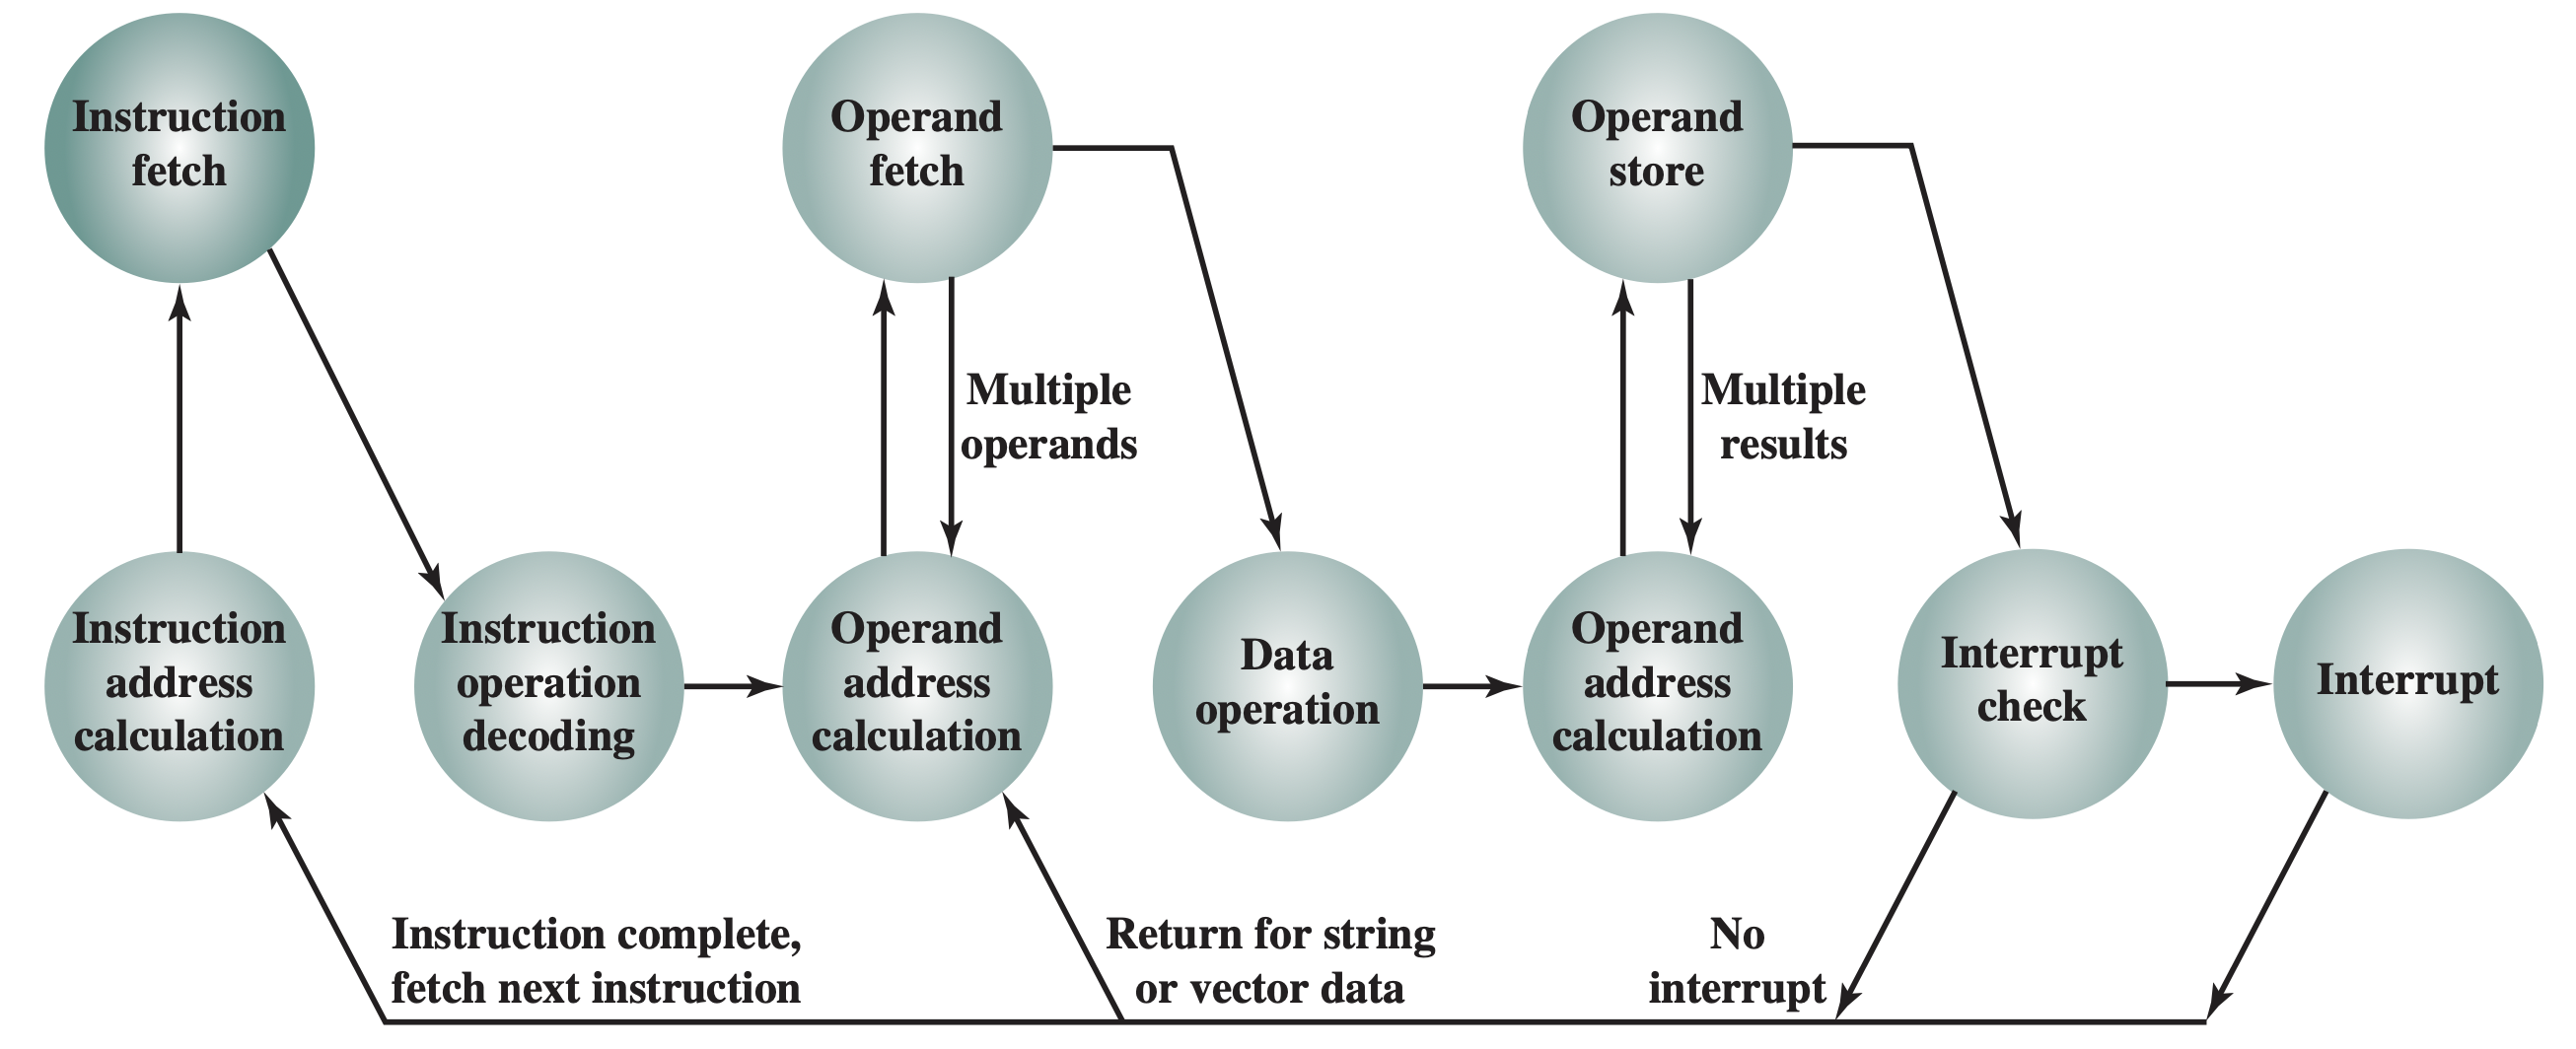
\includegraphics[width=0.85\textwidth]{chaps/instruction-execution-cycle/instruction-cycle-interrupts.png}
    \caption{Instruction Execution Cycle with Interrupts Handling}
\end{figure}

\subsubsection{Instruction Format}

An instruction can be one-word or multi-word. A typical form of instruction may have the
format of:
\begin{table}[H]
    \centering
    \begin{tabular}{cccc}
        Byte 0                       & Byte 1                                & Byte 2                                & Byte 3                                   \\ \hline
        \multicolumn{1}{|c|}{Opcode} & \multicolumn{1}{c|}{Source Operand 1} & \multicolumn{1}{c|}{Source Operand 2} & \multicolumn{1}{c|}{Destination Operand} \\ \hline
    \end{tabular}
\end{table}
where opcode stands for operation code, for example, \texttt{ADD (0x00)}, \texttt{SUB (0x01)},
\texttt{AND (0x02)}, \texttt{OR (0x03)}, \texttt{NOT (0x04)} etc.

\begin{enumerate}

\item \textbf{Arithmetic and Logical Operations}:

Consider this operation: \texttt{ADD R1, R2, R3} (or in pseudocode, \texttt{R3 = R1 + R2}),
the instruction is represented as \texttt{0x00010203}. Since \texttt{ADD} requires two source
operands and one destination operand, all fields are used.

Consider \texttt{NOT R1, R2} (or in pseudocode, \texttt{R2 = NOT R1}), the instruction is
represented as \texttt{0x04010002}. Since \texttt{NOT} uses only one source operand, the
second source operand is set as \texttt{0x00}.

\item \textbf{\texttt{LD} and \texttt{ST} Instructions}:

For instructions that uses memory, a two-word instruction is needed as the memory address
cannot fit in the operand. Assume that \texttt{LD (0x06)} and \texttt{ST (0x07)}.
For example, \texttt{LD P1(0x0000003c), R1}, which loads the content of
memory address \texttt{P1} to register \texttt{R1}, the instruction is represented as
\texttt{0x0600ff01 0000003c}. The format is:
\begin{table}[H]
    \centering
    \begin{tabular}{ccccclll}
    Byte 0                       & Byte 1                                     & Byte 2                                      & Byte 3                                   & Byte 4    & Byte 5    & Byte 6    & Byte 7   \\ \hline
    \multicolumn{1}{|c|}{Opcode (\texttt{LOAD})} & \multicolumn{1}{c|}{Source (\texttt{0x00})} & \multicolumn{1}{c|}{Addressing Mode (\texttt{0xff})} & \multicolumn{1}{c|}{Destination} & \multicolumn{4}{c|}{Memory Address} \\ \hline
    \multicolumn{4}{c}{Word 0}                                                                                                                                         & \multicolumn{4}{c}{Word 1}                  
    \end{tabular}
\end{table}

\begin{remark}
    For simplicity, there is only one addressing mode (\texttt{0xff}) used in this section.
\end{remark}

\item \textbf{Branching Instructions}:

A branching instruction has the following format:
\begin{table}[H]
    \centering
    \begin{tabular}{ccccclll}
    Byte 0                                & Byte 1                              & Byte 2                                         & Byte 3                          & Byte 4     & Byte 5     & Byte 6     & Byte 7    \\ \hline
    \multicolumn{1}{|c|}{Opcode (Branch)} & \multicolumn{1}{c|}{Condition Code} & \multicolumn{1}{c|}{Address/Addressing Mode} & \multicolumn{1}{c|}{(not used)} & \multicolumn{4}{c|}{Address of Destination Instruction} \\ \hline
    \multicolumn{4}{c}{Word 0}                                                                                                                                     & \multicolumn{4}{c}{Word 1}                      
    \end{tabular}
\end{table}

Examples of condition codes are:
\begin{table}[H]
    \centering
    \begin{tabular}{|c|c|l|}
    \hline
    \textbf{Instruction} & \textbf{Condition Code} & \textbf{Meaning} \\ \hline
    \texttt{BR} & \texttt{0x00} & Unconditional branch \\ \hline
    \texttt{BZ} & \texttt{0x01} & Branch if zero \\ \hline
    \texttt{BNZ} & \texttt{0x02} & Branch if not zero \\ \hline
    \end{tabular}
\end{table}
By saying ``zero'', it means to check the zero flag of the ALU to determine if the previous
operation resulted in zero. Other flags may also be used.

\begin{example}
    Consider this code (on the right side is the machine code in hexadecimal):
    \begin{minted}[style=friendly]{asm}
        LD  P2, R2      ;                       0000: 0600ff02 00000034
        LD  P1, R1      ;                       0008: 0600ff01 00000030
        LD  P3, R3      ;                       0010: 0600ff03 00000038
        MOV R2, R4      ;                       0018: 05020004
    L:  ADD R2, R3, R2  ; Increment R2 by 1     001C: 00020302
        SUB R1, R2, R4  ; R4 = R1 - R2          0020: 01010204
        BNZ L           ; If R4 != 0, go to L   0024: 0802ff00 0000001C
        HLT             ;                       002C: 09000000 
    P1: .WORD 5         ;                       0030: 00000005
    P2: .WORD 0         ;                       0034: 00000000
    P3: .WORD 1         ;                       0038: 00000001
    P:  .WORD           ;                       003C: 00000000
    \end{minted}
    The \texttt{BNZ} instruction is used to create a loop that increments \texttt{R2} by 1
    until \texttt{R1 - R2} is zero. The program halts when the condition is met.
\end{example}

\item \textbf{Halt Instruction}:

The \texttt{HLT} instruction is used to halt the program. It does not use any operands
and those fields are set to \texttt{0x00}.

\end{enumerate}

\subsubsection{Instruction Fetch}

Address to the next instruction is stored in PC register, which is incremented automatically
during execution. For a two-word instruction, the first word is fetched first, then PC
is incremented by 1 word to point to the second word. Then the second word is fetched,
and PC is incremented again to point to the next instruction.

Note that PC is will be changed when branching happens.

This process is called Instruction Address Calculation (IAC).

During IF, the following data transfer happens:
\begin{align*}
    \text{MAR} &\leftarrow \text{PC} \\
    \text{PC} &\leftarrow \text{PC} + 1 \\
    \text{MBR} &\leftarrow \text{Memory}[\text{MAR}]
\end{align*}

\subsubsection{Instruction Decode}

The control unit will decode the instruction and setup the ALU and other components
for appropriate operations (e.g. memory read/write, data transfer, etc.). These actions
are carried out at appropriate times by the control unit.

\subsubsection{Operand Fetch}

If the operands are in registers, data are moved from registers to ALU.

If the operands are in memory, then the instruction would be a two-word instruction.
Note that if PC points to the second word of a two-word instruction, after the above process,
MBR will contain the \textbf{address} of the second word, not the content. Therefore, another
memory read is needed to fetch the content, by:
\begin{align*}
    \text{MAR} &\leftarrow \text{MBR} \\
    \text{MBR} &\leftarrow \text{Memory}[\text{MAR}]
\end{align*}

\subsubsection{Execution}

The ALU performs the operation specified by the instruction. The result is stored in
some temporary register.

\subsubsection{Result Store}

Similar to operand fetch, if the destination is in register, RF write is performed.
If the destination is in memory, then operand address calculation is first performed.
Then the data is written to memory.

\subsubsection{Interrupt Handling}

Interruptions are important as:
\begin{itemize}
    \item They improve efficiency.
    \item When an I/O arrives, it may need immediate attention, or data may be lost.
        e.g. incoming data from a network.
    \item Other programs may also need the CPU's attention. e.g. on a time-sharing system.
\end{itemize}

When interruption is required, I/O device sends a signal to the CPU. The CPU will need to
remember the current state of the program, and then jump to serve the interrupt. The CPU
will then return to the original program and continue execution as if nothing happened.

Interrupt handlers can either be hardware or software.

Interrupt signals are checked at the end of one complete instruction cycle, minimising the
registers that need to be saved/restored. Before each interrupt, the following information
is saved (by pushing to the stack):
\begin{itemize}
    \item Flag register -- to remember the state of the ALU.
    \item PC -- to remember the address of the next instruction.
    \item Modified register files.
    \item The current address of the instruction -- to remember where the program was
        interrupted, while the address of the interruption program is loaded to PC.
\end{itemize}
Other registers (like MAR, MBR, IOAR, etc.) are not saved as they are only meaningful
during the current instruction cycle.

\section{Memory}

\subsection{Memory Hierarchy}

Different types of memory exhibit different performance and impose different costs
of production. To achieve a balance between performance and cost, a hierarchy of
memory is introduced.

\begin{enumerate}
    \item \textbf{Inbound Memory}: The fastest memory in the hierarchy.
    \begin{itemize}
        \item \textbf{Registers}: inside the processor.
        \item \textbf{On-chip Cache}: on the CPU chip.
        \item \textbf{Cache Memory}: on the motherboard.
        \item \textbf{Main Memory}: RAM, on the motherboard.
    \end{itemize}
    \item \textbf{Outbound Storage}: Secondary memory. e.g. hard disk, SSD, DVD, etc.
    \item \textbf{Off-line Storage}: magnetic tapes, etc.
\end{enumerate}

Going from top to bottom, we observe the following trends:
\begin{itemize}
    \item \textbf{Capacity}: increases.
    \item \textbf{Cost per bit}: decreases.
    \item \textbf{Access time}: increases.
    \item \textbf{Frequency of access}: decreases.
\end{itemize}

\subsubsection{Principle of Locality}

\begin{definition}[Principle of Locality]
    The Principle of Locality states that programs do not access all memory locations
    uniformly. Some memory locations have higher tendency to be accessed than others.
\end{definition}

There are two types of locality:
\begin{definition}[Temporal Locality]
    If a memory location is accessed, it is likely to be accessed again soon.
\end{definition}

\begin{definition}[Spatial Locality]
    If a memory location is accessed, it is likely that nearby memory locations
    will be accessed soon.
\end{definition}

\begin{example}
    Consider the following code:
\begin{minted}[style=friendly]{cpp}
    for (int i = 0; i < 100; i++) {
        sum += arr[i];
            // sum is accessed in every iteration -> temporal locality
            // consecutive memory locations of arr[] are accessed -> spatial locality
    }
\end{minted}
\end{example}

\subsubsection{Memory Organisation}

For multi-byte data, they are stored differently in memory on different architectures.
\begin{itemize}
    \item \textbf{Big Endian Mode}: Stored in memory from left to right. (e.g. IBM mainframes)
    \item \textbf{Little Endian Mode}: Stored in memory from right to left. (e.g. Intel x86)
\end{itemize}

\begin{example}
    For storing the 4-byte integer \texttt{0x12345678} in memory:
    \begin{table}[H]
        \centering
        \begin{tabular}{rcccc}
        Address                            & \texttt{101}                     & \texttt{102}                     & \texttt{103}                     & \texttt{104}                     \\ \cline{2-5} 
        \multicolumn{1}{r|}{Big Endian}    & \multicolumn{1}{c|}{\texttt{12}} & \multicolumn{1}{c|}{\texttt{34}} & \multicolumn{1}{c|}{\texttt{56}} & \multicolumn{1}{c|}{\texttt{78}} \\ \cline{2-5} 
        \multicolumn{1}{r|}{Little Endian} & \multicolumn{1}{c|}{\texttt{78}} & \multicolumn{1}{c|}{\texttt{56}} & \multicolumn{1}{c|}{\texttt{34}} & \multicolumn{1}{c|}{\texttt{12}} \\ \cline{2-5} 
        \end{tabular}
    \end{table}
\end{example}

\subsubsection{Unit of Transfer}

CPU reads data not from main memory but from cache memory, as main memory is
much slower. Between cache and main memory, data are transferred in blocks, which
contain multiple bytes (e.g. 4 KBytes).

\subsubsection{Access Methods}

\begin{enumerate}
    \item \textbf{Sequential Access}: Data is accessed from the beginning to the end.
    \item \textbf{Random Access}: Data can be accessed in any order directly, by
        providing the address. Has a constant latency.
    \item \textbf{Associative Access}: Data can be accessed by providing the content
        of the data, not the address. Used in cache memory and Content-Addressable
        Memory (CAM).
\end{enumerate}

\subsection{Internal Memory}

This section presents some common CMOS\footnote{Complementary Metal-Oxide-Semiconductor} memory
technologies and their characteristics.

\subsubsection{Read-Only Memory (ROM)}

\begin{itemize}
    \item Fabricated like integrated circut chips.
    \item Non-volatile memory, i.e., retains data even when power is turned off.
    \item \textbf{Programmable ROM (PROM)}: Can be programmed once. Usually done by supplier
        or customer after chip is manufactured.
    \item Content cannot be changed.
\end{itemize}

\subsubsection{Read-Mostly Memory}

\begin{itemize}
    \item \textbf{Erasable Programmable ROM (EPROM)}: Can be erased and reprogrammed multiple times.
        Erasing is done by exposing the chip to ultraviolet light for a specified time.
    \item \textbf{Electrically Erasable PROM (EEPROM)}: Can be erased and reprogrammed in place.
        Only the bytes addressed are changed. Erasing process is slow.
\end{itemize}

\subsubsection{Flash Memory}

\begin{itemize}
    \item Non-volatile memory.
    \item Between EPROM and EEPROM.
    \item Faster write than EEPROM.
    \item Have limited number of write cycles.
    \item Usage: USB drives, SSD, storage of BIOS (in recent years).
\end{itemize}

\subsubsection{Random Access Memory (RAM)}

\begin{table}[H]
    \centering
    \begin{tabular}{|l|l|l|}
    \hline
    \textbf{Characteristic} & \textbf{Dynamic RAM}                          & \textbf{Static RAM}        \\ \hline
    Storage Technology      & Use transistors to store electric charges.    & Use logic gates (latches). \\ \hline
    Refreshing              & Required (every few ms due to leaking charge) & Not required               \\ \hline
    Speed                   & Slower (delay due to capacitance)             & Faster                     \\ \hline
    Usage                   & Main memory                                   & Cache memory               \\ \hline
    Cost                    & Cheap                                         & Very expensive             \\ \hline
    \end{tabular}
\end{table}

\subsubsection{Comparison of Memory Types}

\begin{table}[H]
    \centering
    \begin{tabular}{|l|l|l|l|l|}
    \hline
    \textbf{Memory Type} & \multicolumn{1}{c|}{\textbf{Category}} & \multicolumn{1}{c|}{\textbf{Erasure}}                               & \multicolumn{1}{c|}{\textbf{\begin{tabular}[c]{@{}c@{}}Write\\ Mechanism\end{tabular}}} & \multicolumn{1}{c|}{\textbf{Volatility}} \\ \hline
    RAM                  & Read-write                             & \begin{tabular}[c]{@{}l@{}}Electrically,\\ byte-level\end{tabular}  & Electrically                                                                            & Volatile                                 \\ \hline
    ROM                  & \multirow{2}{*}{Read-only}             & \multirow{2}{*}{Not possible}                                       & Masks                                                                                   & \multirow{5}{*}{Nonvolatile}             \\ \cline{1-1} \cline{4-4}
    PROM                 &                                        &                                                                     & \multirow{4}{*}{Electrically}                                                           &                                          \\ \cline{1-3}
    EPROM                & \multirow{3}{*}{Read-mostly}           & \begin{tabular}[c]{@{}l@{}}UV light,\\ chip-level\end{tabular}      &                                                                                         &                                          \\ \cline{1-1} \cline{3-3}
    EEPROM               &                                        & \begin{tabular}[c]{@{}l@{}}Electrically,\\ byte-level\end{tabular}  &                                                                                         &                                          \\ \cline{1-1} \cline{3-3}
    Flash                &                                        & \begin{tabular}[c]{@{}l@{}}Electrically,\\ block-level\end{tabular} &                                                                                         &                                          \\ \hline
    \end{tabular}
\end{table}

\subsubsection{Benchmarking Memory Performance}

Key metrics for memory performance include:
\begin{itemize}
    \item \textbf{Access Time}: Time taken to read/write data.
    \item \textbf{Bandwidth/Transfer Rate}: Rate at which data can be read/written.
    \item \textbf{Memory Cycle Time}: ($\text{Access Time} + \text{Transfer Time}$).
\end{itemize}

\begin{example}
    A two-level memory system has an upper level with $0.01\mu \text{s}$ access time and
    a lower level with $0.1\mu \text{s}$. The upper level has a hit rate of $95\%$. The
    average time to access memory is:
    \begin{equation*}
        0.01 \times 0.95 + (0.01 + 0.1) \times 0.05 = 0.015\mu \text{s}
    \end{equation*}
\end{example}

\subsubsection{Error Detection and Correction}

Errors may arise from various sources such as spike in voltage (lightning), electromagnetic
interference (cosmic ray), power supply problems, etc. Extra bits are required to detect errors.
(Usually in secondary storage devices but not in main memory as it is volatile and less likely
to have errors.)

Common error detection and correction methods include:
\begin{itemize}
    \item \textbf{Parity Bit}: Extra bit added to data to make number of 1s even/odd.
        (Cannot be used to correct errors. Cannot detect 2$n$-bit errors.)
    \item \textbf{Hamming Code}
    \item \textbf{Repetition Code}
\end{itemize}

\subsection{Cache Memory}

Cache memory is transparent (hidden) to the software and is managed by the hardware.
It stores copies of frequently accessed data to speed up subsequent access to that data.

There can be one or more layers between the CPU and main memory.
The transfer between the CPU and L1 cache is the fastest, and the speed decreases
as the distance from the CPU increases.

\subsubsection{Cache Memory Organisation}

A word-addressable main memory with $n$-bit addresses has $2^n$ words. Divide the
main memory into blocks of $K$ words each, then the memory has $M=\frac{2^n}{K}$ blocks.
Suppose the cache has $m$ blocks, called \textbf{lines}. Generally, we have $m \ll M$.
Each line has $K$ words, a tag, and several control bits. The length of the line,
excluding the tag and the control bits is called the \textbf{line size} or
\textbf{block length}.

\begin{figure}[H]
\centering
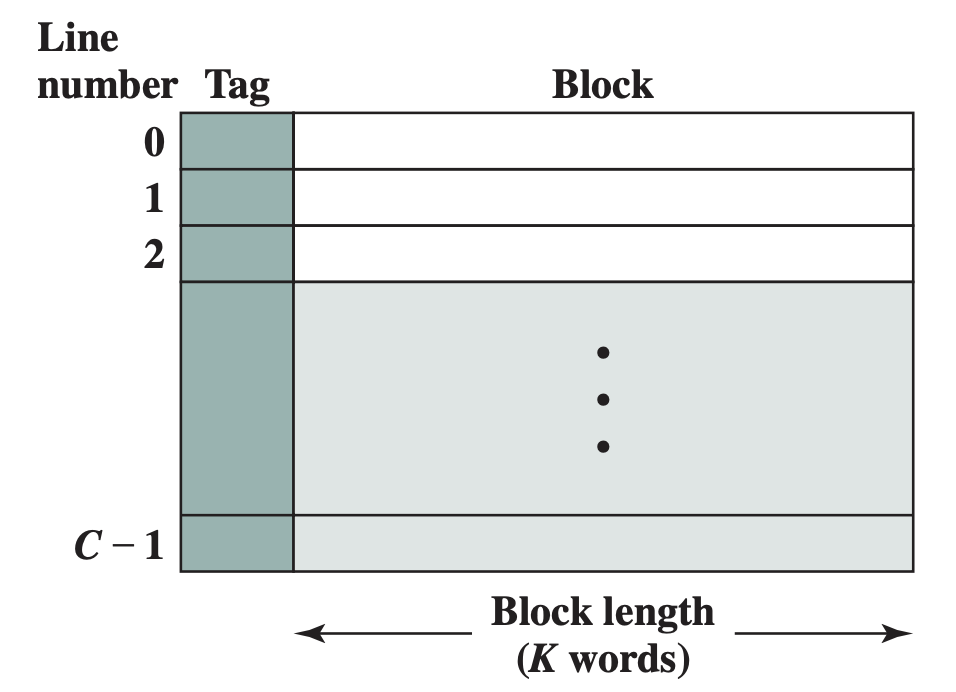
\includegraphics[width=0.4\linewidth]{chaps/memory/cache-memory/cache-mem-organisation.png}
\caption{Cache Memory Organisation}
\end{figure}

\subsubsection{Cache Memory Read}

The process of reading from the cache is roughly described as follows:
\begin{enumerate}
    \item Obtain the address of the word to be read from the CPU.
    \item Check if the block containing the word is in the cache.
    \begin{enumerate}
        \item If the block is in the cache, read the word from the cache.
        \item If the block is not in the cache, load the block from the main memory
            into the cache, and \textbf{at the same time} deliver the word to the CPU.
    \end{enumerate}
\end{enumerate}

\subsubsection{Address Mapping}

There are three ways to map the main memory to the cache:
\begin{enumerate}
\item \textbf{Direct Mapping}: 
    Each block of main memory maps to exactly one line in the cache. The mapping is
    given as 
    \[i = j \bmod m\]
    where $i$ is the cache line number, $j$ is the main memory
    block number, and $m$ is the number of cache lines.
    
    \begin{example}
        The cache logic treats the main memory address in three parts as follows:
        \begin{equation*}
            \underbrace{
            \overbrace{0000\,0001}^{(s-r)\text{ bits (tag)}}\,
            \overbrace{1111\,1111\,1111\,11}^{r\text{ bits (line number)}}}
            _{\text{block number}}
            \overbrace{00}^{w\text{ bits (word)}}
        \end{equation*}
        The least significant $w$ bits identify the word within the block,
        where the block size is $2^w$ words. The next $r$ bits identify the line
        number within the cache memory, where the cache memory has $2^r$ lines.
        The most significant $(s-r)$ bits are the tag bits, which are used to
        distinguish between the different main memory blocks that map to the same line,
        where the main memory has $2^s$ blocks.
    \end{example}

    To perform a read operation, the line number first identifies the line in the cache.
    Then, the tag bits in the line are compared with the tag bits in the address.
    If the tags match, the word is read from the cache according to the word bits in the
    address. If the tags do not match, the block is read from the main memory into the
    cache, and the word is read from the cache.

    \begin{multicols}{2}
        \textbf{Advantages}: \begin{itemize}
            \item Only need to check one cache line, fast.
            \item No selection is required, less use of logic gates, inexpensive.
        \end{itemize}
        \columnbreak
        \textbf{Disadvantages}: \begin{itemize}
            \item When two blocks map to the same line are accessed alternatively,
                constant cache misses occur.
            \item The cache is not fully utilised.
        \end{itemize}
    \end{multicols}

\item \textbf{Fully Associative Mapping}:
    Any block of main memory can be loaded into any line of the cache. The main memory
    address is treated as two parts only -- the tag and the word bits. Again, for a main
    memory address of $(s+w)$ bits, and a cache memory with block length of $2^w$ words,
    the word bits are the least significant $w$ bits, and the tag bits are the remaining
    $s$ bits.

    To perform a read operation, the cache controller searches the entire cache for the
    desired tag. If it is a miss, the block is read from the main memory into the cache.

    \begin{multicols}{2}
        \textbf{Advantages}: \begin{itemize}
            \item More flexible use of cache than direct mapping.
            \item Higher hit rate.
        \end{itemize}
        \columnbreak
        \textbf{Disadvantages}: \begin{itemize}
            \item Requires more complex logic and circuits for tag comparison, more expensive.
            \item Must simultaneously search all cache lines, slower.
        \end{itemize}
    \end{multicols}

\item \textbf{Set Associative Mapping}:
    The cache consists of a number of sets, and each sets consists of a number of lines.
    Their relationship is given by
    \begin{align*}
        m &= v \times k \\
        i &= j \bmod v
    \end{align*}
    where $i$ is the set number, $j$ is the main memory block number, $m$ is the number
    of lines in cache, $v$ is the number of sets, and $k$ is the number of lines in each set.
    ($k$ is usually 2, the maximum is 8.) Also referred to as $k$-way set associative mapping.

    Block $B_j$ in main memory maps to any of the lines in set $j$ in the cache. There are
    two ways of implementing a set associative mapping, either as
    \begin{enumerate}
        \item $v$ associative-mapped caches 
            (usually used for high associativity, i.e. larger $k$).
            Each cache is called a \textbf{set}.
        \item $k$ direct-mapped caches (for lower associativity).
            Each cache is called a \textbf{way}.
    \end{enumerate}

    The cache control logic treats the $(s+w)$-bit main memory address in three parts:
    tag, set, and word.
    The $d$ bits of set identifies the set in cache, where $v = 2^d$.
    The least significant $w$ bits identify the word.
    The remaining $(s-d)$ bits are the tag bits.

    With this method, the tag size is much smaller than in fully associative mapping,
    and each tag is only compared with $k$ tags in a single set.

    \begin{multicols}{2}
        \textbf{Advantages}: \begin{itemize}
            \item Fewer misses than direct mapping.
        \end{itemize}
        \columnbreak
        \textbf{Disadvantages}: \begin{itemize}
            \item Complex selection and comparison logic, slightly slower.
        \end{itemize}
    \end{multicols}

\end{enumerate}

\begin{example}
    Suppose a computer has a byte-addressable main memory with addresses of 32 bits,
    a 64 KB 2-way set associative cache memory, and the block size is 128 bytes. Find
    the number of bits in the tag, set, and word fields of the main memory address.

    \begin{solution}
    Since the block size is 128 ($2^7$) bytes, then the word field is 7 bits.

    Number of blocks in cache memory is $64 \times 2^{10} \div 2^7 = 512$ blocks.

    Number of sets in cache memory is $512 \div 2 = 256 = 2^8$ sets. Therefore, the set
    field is 8 bits.

    The remaining bits are the tag field, which is $32 - 8 - 7 = 17$ bits.

    \begin{table}[H]
        \centering
        \begin{tabular}{|c|c|c|}
            \hline
            \textbf{Tag} & \textbf{Set} & \textbf{Word} \\ \hline
            17 & 8 & 7 \\ \hline
        \end{tabular}
    \end{table}
    \end{solution}
\end{example}

\subsubsection{Replacement Algorithms}

When all lines are occupied and a new block needs to be loaded into the cache, a line
must be selected to be replaced. The different replacement algorithms are:
\begin{enumerate}
\item \textbf{Random Replacement} (RR): 
    A random line is selected to be replaced. This is the simplest method, but it
    does not guarantee the best performance. Not used in practice.

\item \textbf{First-In-First-Out} (FIFO):
    The line that has been in the cache the longest is replaced. It does not consider
    the frequency of use of the block.

\item \textbf{Least Recently Used} (LRU):
    The line that has not been used for the longest time is replaced.

\item \textbf{Least Frequently Used} (LFU):
    The line that has the fewest references is replaced, often implemented with a counter.
\end{enumerate}

Note that replacement algorithms do not apply to direct-mapped caches, as there is only
one possible line to replace.

\subsubsection{Write Policies}

To maintain consistency between the cache and main memory, the main memory must be updated
whenever the cache line to be replaced has been modified. There are two write policies:
\begin{enumerate}
\item \textbf{Write-Through}:
    The main memory is updated whenever the cache is updated. This ensures that the main
    memory is always up-to-date, but it is slower as the CPU must wait for the main memory
    to be updated.

\item \textbf{Write-Back}:
    The line is associated with a \textbf{dirty bit} that is set whenever the line is
    modified. The main memory is only updated when the line is replaced and the dirty bit
    is set. This method minimises the number of main memory writes and is faster.
    The main drawback is that the main memory may be inconsistent.
\end{enumerate}

\subsubsection{Performance}

\begin{definition}[Average Access Time]
    The average access time of a cache memory is given by
    \begin{align*}
        \text{Average Access Time}
        &= \text{Hit Rate} \times \text{Hit Time} + \text{Miss Rate} \times \text{Average Time When Miss} \\
        &= \text{Hit Time} + \text{Miss Rate} \times \text{Miss Penalty}
    \end{align*}
\end{definition}

\begin{example}
    Assume the access time of main memory is 50 ns, the L1 cache has a miss rate and access
    time of 10\% and 1 ns, respectively, the L2 cache has a miss rate and access time
    of 5\% and 5 ns, respectively, and the L3 cache has a miss rate and access time of 2\%
    and 10ns, respectively. Calculate the average access time of the memory system.

    \begin{solution}
        When there is no cache, access time $=50$ ns.

        When there is only L1 cache, access time $=1+10\%\times 50=6$ ns.

        When there are L1 and L2 caches, access time $=1+10\%\times(5+5\%\times 50)=1.75$ ns.

        When there are L1 to L3 caches, access time $=1+10\%\times(5+5\%\times(10+2\%\times 50))=\boxed{1.555\text{ ns}}$.
    \end{solution}
\end{example}

\begin{example}
    Consider a hypothetical machine with 512 words of cache memory. They are in two-way
    set associative organisation, with cache block size of 64 words, using LRU replacement.
    Suppose the cache hit time is 8 ns, and the time to transfer the first word from main
    memory to cache is 60 ns, while subsequent words require 10 ns each. 
    \begin{enumerate}
        \item What is the cache miss penalty?
        \item If there is a read sequence of 28 blocks accessed that has 15 cache misses,
            what is the cache hit rate?
        \item What is the average memory access time?
    \end{enumerate}

    \begin{solution}
    \begin{enumerate}
        \item Cache miss penalty is the time to transfer one block from main memory to cache.
            $60+63\times10=\boxed{690\text{ ns}}$
        \item Cache hit rate $=1-\frac{15}{28\times32}=\boxed{98.33\%}$.
        \item Average memory access time $=8+(1-0.9833)\times690=\boxed{19.52\text{ ns}}$.
    \end{enumerate}
    \end{solution}
\end{example}

\subsection{External Memory}

\subsubsection{Hard Disk Drives (HDD) - Magnetic Disks}

\begin{figure}[H]
    \centering
    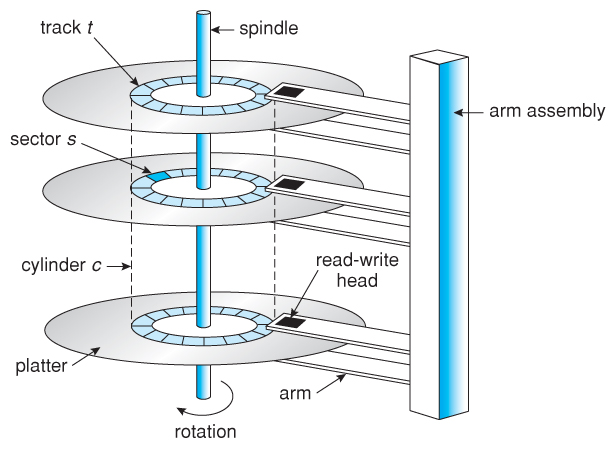
\includegraphics[width=0.58\textwidth]{chaps/memory/external-memory/hdd-layout.jpg}
    \caption{Disk Data Layout}
\end{figure}

\textbf{Terminologies about the HDD layout and components}:
\begin{itemize}
    \item \textbf{Platter}: Magnetically coated disks.
    \item \textbf{Track}: Concentric rings on a platter.
    \item \textbf{Sector}: A segment of a track, usually 512 bytes.
    \item \textbf{Cylinder}: Tracks of different platters that are under the read/write head
        at the same time.
\end{itemize}

\textbf{Formats of Tracks} -- Tracks contain sectors that hold data and other bits that
are useful for the disk controller. The example of a track format can be:
\begin{itemize}
    \item Each track contains 30 sectors of fixed-length 600 bytes, with 512 bytes for data
        and 88 bytes for control information.
    \item Each sector contains several fields: \begin{itemize}
        \item \textbf{Gap 1} (17 bytes): Used to separate sectors.
        \item \textbf{ID Field}: Contains Synch (1 byte), Track, Head, Sector \# (4 bytes),
            and CRC (2 bytes).
        \item \textbf{Gap 2} (41 bytes): Used to separate ID field and data field.
        \item \textbf{Data Field} (515 bytes): Contains 1 Synch byte, 512 bytes of data, and 2
            CRC bytes.
        \item \textbf{Gap 3} (40 bytes)
    \end{itemize}
\end{itemize}

\begin{wrapfigure}{l}{0.6\textwidth}
    \centering
    \begin{subfigure}{0.28\textwidth}
        \centering
        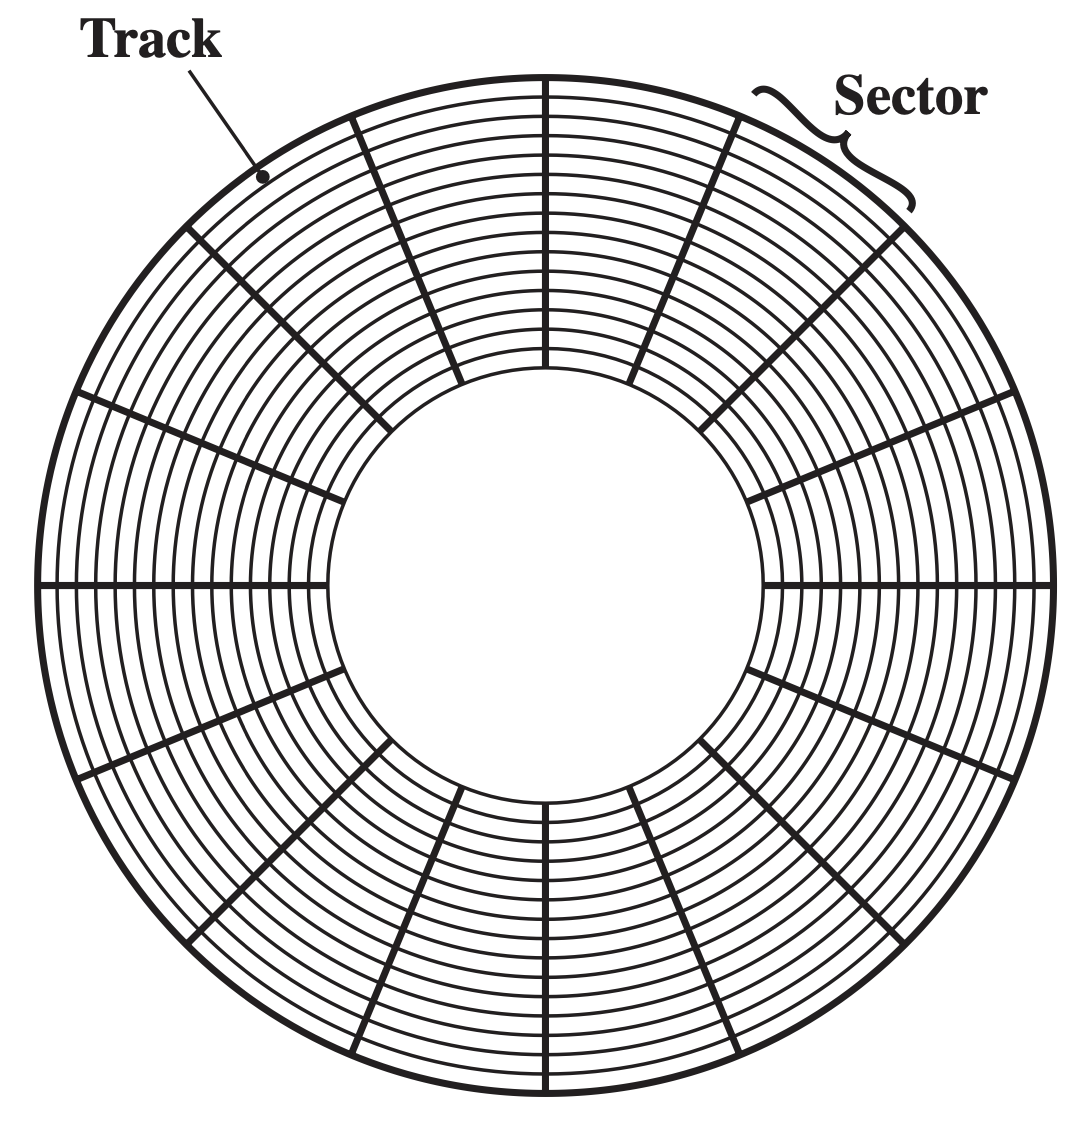
\includegraphics[width=\textwidth]{chaps/memory/external-memory/disk-layout-cav.png}
        \caption{CAV}
    \end{subfigure}
    \hfill
    \begin{subfigure}{0.28\textwidth}
        \centering
        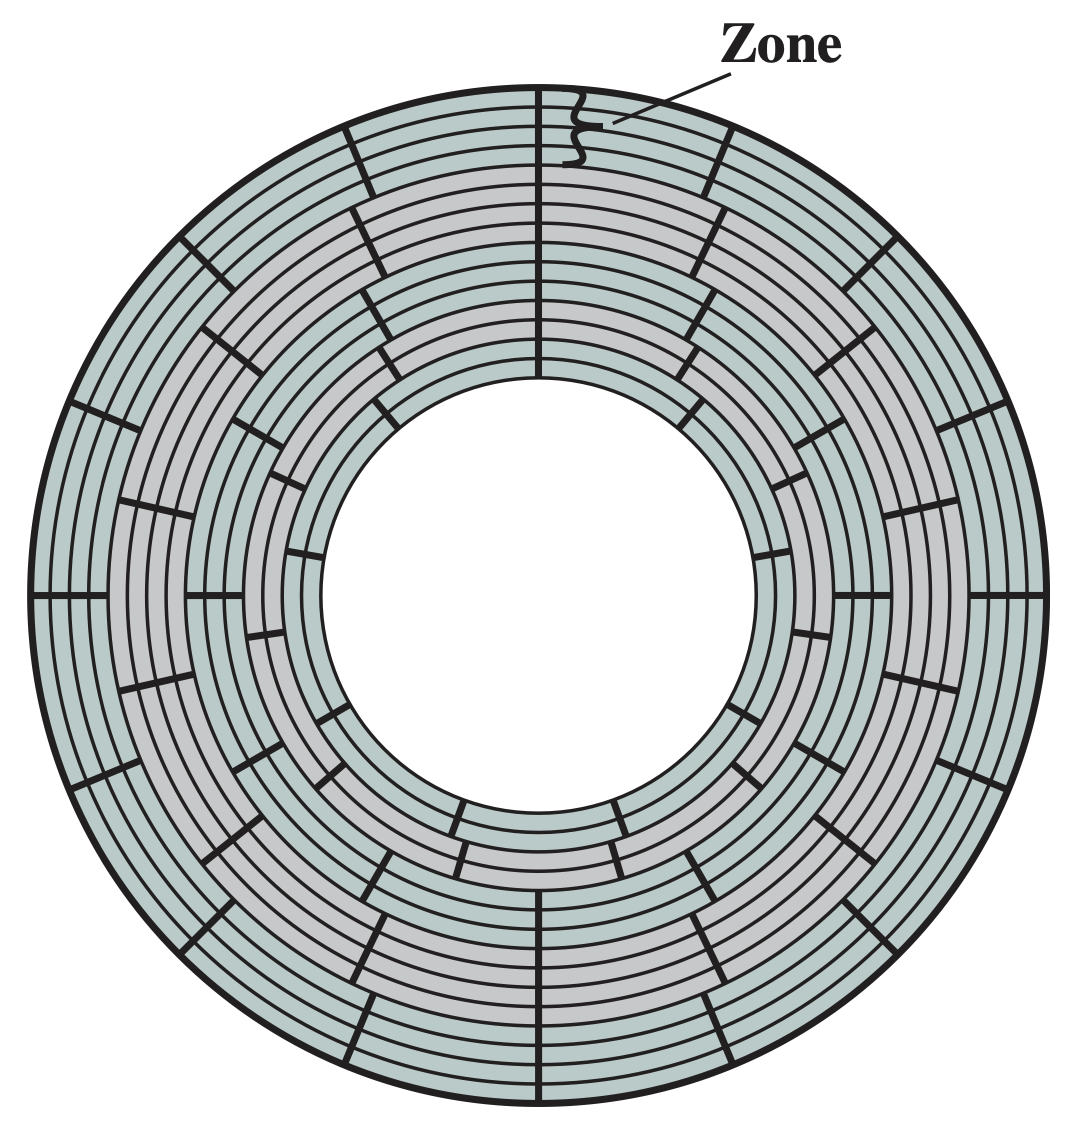
\includegraphics[width=\textwidth]{chaps/memory/external-memory/disk-layout-mzr.png}
        \caption{MZR}
    \end{subfigure}
\end{wrapfigure}

\textbf{Disk Layout Methods}:
\begin{itemize}
    \item \textbf{Constant Angular Velocity (CAV)}: Blocks of data can be directly addressed
        by track and sector. Read/write is easy. However, density of data decreases from the
        inner tracks to the outer tracks, which wastes space.
    \item \textbf{Multiple Zone Recording (MZR)}: Divides the disk into zones, with each zone
        having a different number of sectors per track. Note that the data density is not
        exactly the same, but only approximated to be the same. This allows maximised storage
        capacity.
\end{itemize}

\end{document}